% segmento_es -- el anillo de valores de caracter solo depende del segmento: SU(n), Sp(2m) y
% GL(n) en un elemento de torsion.
% Version en castellano de segmento.tex.  Carles Marin + Claude (asistente IA).
%
% REGLA DE REDACCION: resultados, no proceso.  Lo que se dice de un tercero es lo que esta en un
% articulo suyo, con localizador.  Lo medido va marcado como medido, con su cifra y su rango.
% Las compuertas estan en gates/, con las de las capas de tipo A en gates/capas_tipo/, y el
% cuaderno en ARGUMENTO_TIPOA_2026-09-17.md; cada cifra de aqui sale de una salida archivada.
% No TODAS estan en capas_tipo/: los 462 valores de caracter del bloque del level-rank salen de
% gates/complemento_levelrank_OUT.txt y los coeficientes del residual de
% gates/capas_tipo/qlucas_signo_OUT.txt (hasta el 19-sep esta linea decia lem_unit_B_OUT.txt, que
% trata de otro lema).
%
% TRADUCIR ES REVISAR: la paridad estructural contra el ingles se comprueba con
% herramientas/paridad_segmento.py.  Toda etiqueta, referencia y clave de bibliografia es la
% MISMA que en la version inglesa, a proposito: asi las dos versiones se pueden cotejar linea a
% linea y una figura o un teorema no cambian de nombre al cruzar el idioma.
%
% Compilar:  pdflatex segmento_es (x2).
\documentclass[11pt,a4paper]{article}
\usepackage[T1]{fontenc}
\usepackage[utf8]{inputenc}
\usepackage[spanish,es-noshorthands,es-nodecimaldot,es-tabla]{babel}
\usepackage{lmodern}
\usepackage[margin=2.6cm]{geometry}
\usepackage{amsmath,amssymb,amsthm}
\usepackage{graphicx}
\usepackage{booktabs}
\usepackage[dvipsnames,table]{xcolor}
\usepackage{float}
\usepackage[colorlinks=true,linkcolor=NavyBlue,citecolor=NavyBlue,urlcolor=NavyBlue,
  bookmarksnumbered=true,bookmarksopen=true]{hyperref}
\hypersetup{pdftitle={El anillo de los valores de car\'acter s\'olo depende del segmento},
  pdfkeywords={ordenes generados por valores de caracter, anillo de enteros, indice de un orden,
  grupos de Lie compactos, elementos de orden finito, dualidad nivel-rango, dimensiones cuanticas,
  numero de clases relativo, cuerpos ciclotomicos, ordenes de Gorenstein},
  pdfauthor={Carles Mar\'in}}
\usepackage{microtype}
\usepackage{needspace}
\renewcommand{\topfraction}{0.9}
\renewcommand{\bottomfraction}{0.8}
\renewcommand{\textfraction}{0.07}
\renewcommand{\floatpagefraction}{0.85}


\definecolor{azul}{HTML}{1F4E79}
\definecolor{fondoficha}{HTML}{EEF3F8}
\definecolor{filaclara}{HTML}{F2F6FA}

\newtheorem{theorem}{Teorema}
\newtheorem{proposition}[theorem]{Proposici\'on}
\newtheorem{corollary}[theorem]{Corolario}
\newtheorem{lemma}[theorem]{Lema}
\theoremstyle{definition}
\newtheorem{definition}[theorem]{Definici\'on}
\newtheorem{observation}[theorem]{Observaci\'on}
\newtheorem{question}[theorem]{Pregunta}
\newtheorem{conjecture}[theorem]{Conjetura}
\newtheorem{remark}[theorem]{Observaci\'on}

\newcommand{\Sp}{\mathrm{Sp}}
\newcommand{\SU}{\mathrm{SU}}
\newcommand{\GL}{\mathrm{GL}}
\newcommand{\SO}{\mathrm{SO}}
\newcommand{\SL}{\mathrm{SL}}
\newcommand{\ZZ}{\mathbb{Z}}
\newcommand{\QQ}{\mathbb{Q}}
\newcommand{\FF}{\mathbb{F}}
\newcommand{\cO}{\mathcal{O}}
\newcommand{\cf}{\mathfrak{f}}
\newcommand{\rad}{\mathfrak{r}}
\newcommand{\gr}{\operatorname{gr}}
\definecolor{azulpregunta}{HTML}{1F6FB2}
\newcommand{\frontera}[1]{\par\medskip\noindent{\small\color{azulpregunta}$\triangleright$\ \emph{#1}}\par}
\newcommand{\marco}[1]{{\setlength{\fboxsep}{6pt}\setlength{\fboxrule}{0.6pt}%
  \fcolorbox{azul!45}{fondoficha}{$\displaystyle #1$}}}
\newcommand{\medido}[1]{\emph{Medido}: #1}
\newcommand{\pregunta}[1]{\par\smallskip\noindent\emph{#1}\par\smallskip}

\title{\vspace{-1.4cm}\Large El anillo de los valores de car\'acter s\'olo depende del segmento:\\
$\SU(n)$, $\Sp(2m)$ y $\GL(n)$ en un elemento de torsi\'on}
\author{\normalsize Carles Mar\'in\thanks{Investigador independiente,
\texttt{karlesmarin@gmail.com}. Escrito con Claude (Anthropic) como asistente; v\'ease la
declaraci\'on antes de la bibliograf\'ia.}}
\date{\normalsize\today}

\begin{document}
\maketitle

\begin{abstract}
\noindent
Sea $g_q=\exp(2\pi i\rho/q)$ el elemento principal asociado a $q$ en un grupo simple compacto, y
sea $A$ el anillo generado por todos los valores de car\'acter en $g_q$, un orden en el anillo de
enteros $\cO$ de su cuerpo. Un lema de divisi\'on --- multiplicar un polinomio m\'onico por un
factor entero m\'onico no cambia el anillo que generan sus coeficientes --- da tres operaciones
sobre el segmento de exponentes de los autovalores que dejan $A$ igual: a\~nadir un autovalor $1$,
que hace el anillo de $\SU(2m+1)$ igual al de $\Sp(2m)$; el complemento $n\mapsto q-n$, la dualidad
de nivel-rango como igualdad de \'ordenes; y el per\'iodo $n\mapsto n+q$. As\'i $A$ s\'olo depende
del segmento. En un primo $p$, el \'indice de un segmento estable es la suma de los defectos de
sus capas, y el n\'umero de clases relativo gobierna la primera capa. Un primo $p$ divide a
$[\cO:A]$ s\'olo si la parte $r$ de $q$ prima con $p$ divide a $n-1$, $n$ o $n+1$, y dentro de esas
familias lo hace siempre que $p$ sea un primo impar que divide a $q$ y $\varphi(r)\ge4$. Para el anillo no real de $\GL(n)$, con
$n=Nr$ o $Nr+1$, $2\le n<q$, $r\ge5$ impar y $p$ impar, el orden es localmente una extensi\'on
cuadr\'atica libre del anillo del segmento recentrado.
\end{abstract}

\noindent\textbf{Palabras clave:} \'ordenes generados por valores de car\'acter; anillo de enteros;
\'indice de un orden; grupos de Lie compactos; elementos de orden finito; dualidad nivel--rango;
dimensiones cu\'anticas; n\'umero de clases relativo; cuerpos ciclot\'omicos; \'ordenes de
Gorenstein.

\section{Cincuenta a\~nos de valores, y una pregunta del siglo XIX}

Un valor de car\'acter en un elemento de orden $q$ es una suma de ra\'ices $q$-\'esimas de la
unidad, y en general eso es todo lo que se puede decir. En un elemento se puede decir mucho m\'as,
y se ha dicho tres veces. En 1976 Kostant demostr\'o que en la clase de conjugaci\'on de Coxeter
todo car\'acter irreducible de un grupo compacto simple toma el valor $1$, $0$ o $-1$, y que esos
valores \emph{son} los coeficientes de la identidad de la funci\'on $\eta$ de Macdonald
\cite[Thm.~3.1]{Kostant76}: una sola clase de conjugaci\'on, y una f\'ormula de producto cl\'asica
se lee en ella. Kostant determin\'o m\'as tarde qu\'e pesos contribuyen --- los que tienen
$\lambda+\rho$ en la \'orbita de $\rho$ bajo el grupo de Weyl af\'in en el nivel $\tfrac12$
\cite{Kostant04} --- y Cellini, M\"oseneder Frajria y Papi analizaron esa \'orbita y explicitaron
la descripci\'on, en los tipos cl\'asicos, como un enunciado sobre grupos de Weyl afines
permutando los enteros \cite{CMP}. Y en 2025 Nadimpalli, Pattanayak y Prasad \cite{NPP}
identificaron los propios valores no nulos, para elementos de orden divisor del n\'umero de
Coxeter, como \emph{dimensiones} de representaciones de otro grupo. Cincuenta a\~nos, una pregunta,
tres respuestas cada vez m\'as finas: \emph{\textquestiondown cu\'al es el valor?}

Ahora b\'ajese uno de ese elemento. En cuanto $q$ deja de dividir al n\'umero de Coxeter no hay
descripci\'on de ese tipo, los valores son enteros algebraicos sin forma particular, y pedirlos de
uno en uno deja de ser la pregunta \'util. Preg\'untese en cambio qu\'e \emph{generan}. Fijado
$g_q$, los valores de todos los caracteres en $g_q$ abarcan un cuerpo de n\'umeros y generan dentro
de \'el un subanillo $A$ de \'indice finito en el anillo de enteros $\cO$ --- es decir, un
\emph{orden}, y el invariante que mide un orden tampoco es nuevo. Es el conductor de Dedekind,
introducido en 1877 precisamente para decir cu\'anto dista un orden del maximal y en qu\'e
difieren sus clases de ideales \cite{Ded77}. As\'i que la pregunta \emph{\textquestiondown qu\'e
anillo generan los valores de car\'acter?} es una pregunta decimon\'onica sobre \'ordenes, hecha a
unos generadores que suministra la teor\'ia de representaciones --- y las dos mitades rara vez han
estado en la misma habitaci\'on.

La pregunta misma apenas se ha planteado. Para grupos finitos, B\"achle y Sambale \cite{BS}
demostraron que todo primo que divide al \'indice divide al orden del grupo. Para un grupo de Lie
compacto en un solo elemento de torsi\'on la aplicaci\'on de evaluaci\'on es cl\'asica: Pianzola
estudi\'o el homomorfismo del anillo de representaciones en $\ZZ[\zeta_N]$ que define, y determin\'o
el \emph{cuerpo} que genera mediante un grupo de descomposici\'on en el grupo de Weyl
\cite[Prop.~10, Prop.~13(b)]{Pia87} --- pero no el anillo. El anillo s\'olo lo hemos encontrado
planteado en \cite{Cond}, que calcul\'o el
conductor para $\Sp(2m)$ en sus familias principales --- y encontr\'o que la respuesta es
aritm\'etica y no de teor\'ia de Lie.
El \'indice se lee en una matriz de momentos construida con el diente de sierra de Stickelberger;
sus menores maximales son el \'indice de Sinnott del ideal de Stickelberger \cite{Sin78}, y el
n\'umero de clases relativo $h^-(\QQ(\zeta_{q'}))$ gobierna si la primera capa est\'a llena ---
junto, cuando el segmento cubre per\'iodos enteros, con el factor de Euler $\chi(2)-1$
\cite[Cor.~17]{Cond}, que es el tema de \cite{II}. Esa aritm\'etica es la raz\'on de que los n\'umeros de clases recorran las \S\S\ref{sec:loc}--\ref{sec:sombra}.

Hay una tercera pregunta, y se respondi\'o hace mucho en una habitaci\'on en la que no estaba
ninguna de las otras dos. \emph{\textquestiondown Cu\'ando toman dos grupos distintos los mismos
valores?} Frenkel la plante\'o para \'algebras de Lie afines en 1982 \cite{Fre82}; Pressley y Segal la tienen
como una simetr\'ia $k\leftrightarrow N-k$ de las representaciones de grupos de lazos; Nakanishi y
Tsuchiya la demostraron para los modelos WZW; Witten la dedujo de la \'unica l\'inea de \'algebra
lineal que la hace evidente, $G_V(k,N)\cong G_{V^*}(N-k,N)$ \cite{PS86,NT92,Wit93}. Es la dualidad
nivel-rango, y en cuarenta a\~nos se ha enunciado para \'algebras de fusi\'on, dimensiones
cu\'anticas, bloques conformes, invariantes de nudos y fibrados vectoriales sobre curvas --- y
nunca, hasta donde hemos encontrado, para el anillo que generan los valores.

\'Esa es la forma de esta nota. Las tres preguntas son sobre el mismo objeto, y las respuestas se
apilan una encima de otra: nivel-rango dice \emph{qu\'e} segmentos dan los mismos valores, el carril
del valor dice \emph{cu\'ales} son esos valores, y el conductor dice \emph{qu\'e generan}. El lema
de divisi\'on de la \S\ref{sec:seg} ocupa una l\'inea y cruza los tres: redemuestra el
emparejamiento, a\~nade dos operaciones m\'as que no son emparejamientos, y entrega la respuesta en
la moneda del tercer carril, \'ordenes y conductores. La Figura~\ref{fig:historia} es ese relato
dibujado: tres carriles, cincuenta a\~nos, y la \'unica afirmaci\'on que esta nota hace sobre el
cuadro entero.

\begin{figure}[htbp]
\centering

\includegraphics[width=\textwidth]{fig_historia_es.pdf}
\caption{Tres carriles, cincuenta a\~nos, y esta nota en el cruce. \emph{\textquestiondown Cu\'al es
el valor?} se respondi\'o tres veces, cada vez mejor; el hito central son dos art\'iculos, el
criterio de Kostant de 2004 y su descripci\'on por el Weyl af\'in en los tipos cl\'asicos de 2006.
\emph{\textquestiondown Cu\'ando dan dos grupos los mismos valores?} se respondi\'o entre 1982 y
1993 y es la dualidad nivel-rango; es la Proposici\'on~\ref{prop:ops}(b) de m\'as abajo, dicho de
otro modo. \emph{\textquestiondown Qu\'e anillo generan los valores?} se plante\'o una vez para
grupos finitos y una vez para un grupo compacto. La l\'inea discontinua es lo \'unico que esta nota
afirma sobre el cuadro entero: que los tres carriles son tres vistas de un mismo anillo.}
\label{fig:historia}
\end{figure}

\pregunta{As\'i que: \textquestiondown qu\'e pasa en los dem\'as tipos cl\'asicos?}

La primera respuesta es una coincidencia. El \'indice para $\SU(n)$ da, casilla tras casilla,
\emph{los mismos enteros} que la tabla publicada para $\Sp(2m)$ --- no n\'umeros parecidos, los
mismos. La explicaci\'on ocupa una l\'inea, y es la Proposici\'on~\ref{prop:ops}(a) de m\'as abajo:
los dos anillos son iguales, porque los dos segmentos de autovalores difieren en un solo~$1$, y eso
es un factor entero m\'onico.

Esa coincidencia es el asunto de esta nota. Si dos grupos distintos dan el
mismo anillo,
entonces el anillo no es un invariante del grupo. Es un invariante del \emph{segmento} de exponentes
propios --- y ni siquiera de \'el, sino del segmento salvo tres operaciones expl\'icitas. Una de las
tres es la dualidad nivel-rango, conocida desde hace cuarenta a\~nos; lo que aporta el
Lema~\ref{lem:div} no es demostrar \'esa, sino demostrar las tres a la vez y en una forma --- una
igualdad de \'ordenes --- que la literatura de \'algebras de fusi\'on no tiene motivo para enunciar.
Los grupos cl\'asicos de la recta $\rho$ realizan el mismo bloque de residuos en s\'olo tres
posiciones.

\begin{figure}[htbp]
\centering
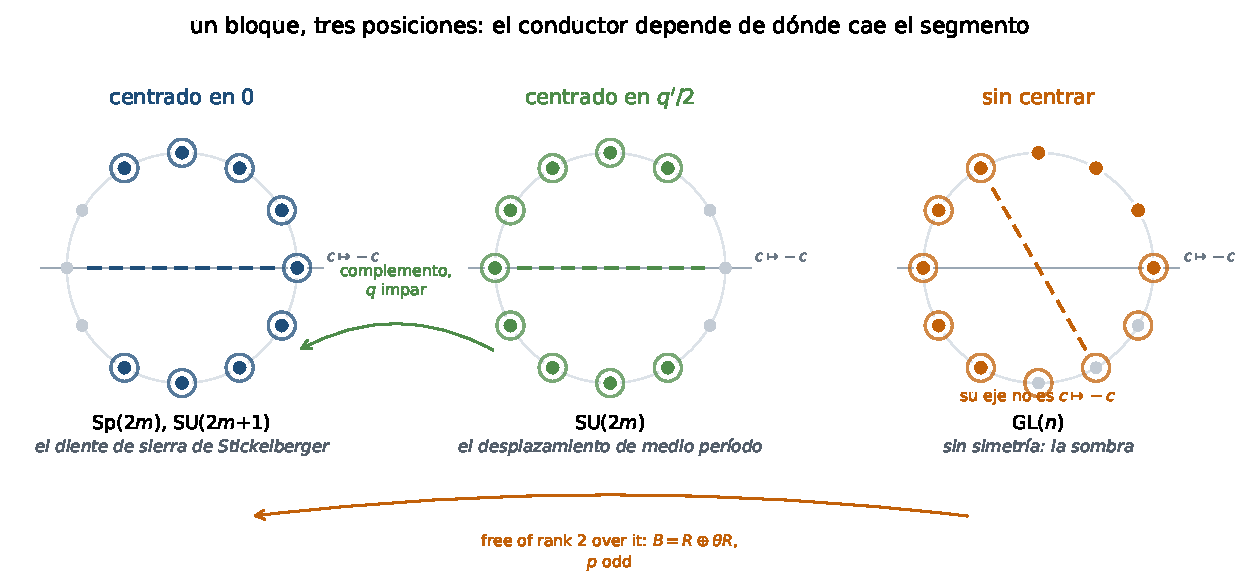
\includegraphics[width=\textwidth]{fig_formas_es.pdf}
\caption{El mismo bloque de residuos, en las tres posiciones que realizan los grupos cl\'asicos. Los
puntos llenos son las clases que ocupa el segmento; los anillos huecos son sus im\'agenes bajo
$c\mapsto-c$; la l\'inea discontinua es el eje propio del bloque, por su punto medio. Cuando el
bloque est\'a centrado en $0$ o en $q'/2$ ese eje es el eje gris $c\mapsto-c$, los anillos caen
sobre los puntos, y el anillo de valores de car\'acter es real; cuando no est\'a centrado los dos
ejes se separan, los anillos se despegan de los puntos, y el anillo no es real. La flecha verde es
el Corolario~\ref{cor:par}: para $q$ impar la posici\'on central no es un r\'egimen aparte, porque
el complemento la lleva a la de la izquierda. La flecha naranja es el Teorema~\ref{obs:puente}, y es
m\'as d\'ebil en especie: la posici\'on derecha no \emph{se convierte} en la izquierda, pero
localmente en un $p$ impar y en las familias $n=Nr,Nr+1$ es una extensi\'on libre de rango $2$ de
ella,
$B=R\oplus\theta R$, donde $R$ es el anillo del segmento recentrado en $Nr/2$ --- un segmento de la
especie de la izquierda. As\'i que las tres posiciones son dos, y la segunda se apoya sobre la
primera.}
\label{fig:formas}
\end{figure}

\pregunta{Si lo que importa es la posici\'on del bloque, \textquestiondown qu\'e posiciones pueden
producir un defecto siquiera, de qu\'e tama\~no es, y qu\'e decide ese tama\~no?}

La tabla las contesta, una fila por secci\'on, y a\~nade la respuesta que la pregunta no
ped\'ia: la posici\'on no centrada tampoco es un r\'egimen propio, sino que se apoya sobre la
primera como extensi\'on libre de grado $2$. Como en \cite{Cond}, un enunciado o est\'a demostrado
o va marcado \emph{medido} con el n\'umero de casillas que lo sostienen; lo que queda abierto va
marcado con $\triangleright$ all\'i donde surge, y las dos cosas que sobreviven a su propia
secci\'on est\'an recogidas al final.

\begin{table}[tb]
\centering\small
\rowcolors{2}{filaclara}{white}
\begin{tabular}{@{}p{0.40\textwidth}p{0.55\textwidth}@{}}
\toprule
pregunta & respuesta \\
\midrule
\textquestiondown Por qu\'e dan dos grupos distintos el mismo anillo? (\S\ref{sec:seg}) &
porque dan el mismo segmento salvo un factor entero m\'onico: tres operaciones, un lema de
divisi\'on. La del medio es la dualidad nivel-rango, conocida desde \cite{PS86,NT92}; las otras dos
no lo son, y el mismo lema demuestra las tres. Lema~\ref{lem:div},
Figura~\ref{fig:operaciones} \\
\textquestiondown Qu\'e aspecto tiene el defecto en un primo? (\S\ref{sec:loc}) &
un \'unico cuerpo residual, una primera capa medida por un m\'odulo c\'iclico, y
cuando $e=2$, $v_p=2\dim-1-W_1$: Teorema~\ref{thm:loc}, Figura~\ref{fig:plano} \\
\textquestiondown Qu\'e primos pueden aparecer? (\S\ref{sec:sop}) &
s\'olo los que cumplen $r\mid n-1,n,n+1$: dentro de las familias el defecto
est\'a forzado en cuanto $\varphi(q')\ge4$ (Proposici\'on~\ref{prop:conv}), fuera de ellas el orden es maximal, por un lema
sobre intervalos de residuos y un recuento de momentos en la primera capa: Lema~\ref{lem:inter},
Proposici\'on~\ref{prop:sop}, Teorema~\ref{thm:sop} \\
\textquestiondown Y cuando el segmento no est\'a centrado? (\S\ref{sec:sombra}) &
el mismo cuadro con la dimensi\'on de la capa duplicada, siendo los generadores binomios gaussianos
torcidos --- y, en las familias $n=Nr,Nr+1$ con $2\le n<q$, una extensi\'on cuadr\'atica libre
$B=R\oplus\theta R$ del anillo del segmento recentrado, con sus capas las de $R$ sumadas a s\'i
mismas desplazadas en $P$ y su tipo igual: Lema~\ref{lem:gauss}, Teorema~\ref{thm:sombra}, Teorema~\ref{obs:puente},
Proposici\'on~\ref{prop:tipopuente}, Figura~\ref{fig:puente} \\
\textquestiondown Por qu\'e aparecen n\'umeros de clases? (\S\S\ref{sec:loc}, \ref{sec:sombra}) &
$h^-$ gobierna si la primera capa est\'a llena --- donde valen las hip\'otesis del
Teorema~\ref{thm:loc} y de la Proposici\'on~\ref{prop:capa1}, y s\'olo como medida en el r\'egimen
par, $q$ par y $p$ impar --- y en la sombra si alcanza su rango de referencia $d+1$, con el
factor de Euler en $2$ como segunda fuente cuando el segmento cubre per\'iodos enteros:
Teorema~\ref{thm:loc}, Proposici\'on~\ref{prop:capa1}, Teorema~\ref{obs:puente} \\
\bottomrule
\end{tabular}
\end{table}

\section{El segmento, y las tres operaciones que preservan el anillo}\label{sec:seg}

Escribamos los autovalores de $g_q$ como $x_j=\zeta_M^{a_j}$. El multiconjunto $\{a_j\}$ es el
\emph{segmento}. Para $\Sp(2m)$ en el elemento principal de tipo $\rho$ es $\{\pm1,\dots,\pm m\}$
con $M=q$. Para $\SU(n)$, con $\rho=\bigl(\tfrac{n-1}{2},\dots,-\tfrac{n-1}{2}\bigr)$, las entradas
son enteras cuando $n$ es impar y semienteras cuando $n$ es par, de modo que
\[
\{-m,\dots,m\}\ \ (n=2m+1,\ M=q),\qquad
\{\pm1,\pm3,\dots,\pm(n-1)\}\ \ (n\ \text{par},\ M=2q).
\]
En los dos casos el segmento es sim\'etrico, as\'i que $g_q$ es conjugado de su inverso y todo valor
de car\'acter es real; $A$ es un orden en el subcuerpo real. Conviene escribir los dos casos sobre
la misma circunferencia: con $t=\zeta_{2q}$ el segmento de $\SU(n)$ es
\[
\marco{\{\,n-1,\ n-3,\ \dots,\ 1-n\,\}\subset\ZZ/2q ,}
\]
$n$ t\'erminos de una clase de paridad m\'odulo $2q$ --- as\'i que para $n$ par $g_q$ tiene orden
$2q$ en $\SU(n)$, y orden $q$ s\'olo en el grupo adjunto; mantenemos $q$ como par\'ametro --- y el
polinomio caracter\'istico de $g_q$ en la representaci\'on est\'andar es $F_{n,q}(T)=\prod_{j=0}^{n-1}\bigl(T-t^{\,n-1-2j}\bigr)$.

Como los caracteres fundamentales de $\SU(n)$ son, salvo un cambio triangular unipotente sobre
$\ZZ$, las funciones sim\'etricas elementales de los autovalores, y $e_n=\prod_jx_j=1$, el anillo
$A$ est\'a generado por los coeficientes de $F_{n,q}$. Todo lo de esta secci\'on es entonces un
enunciado sobre polinomios, y un solo lema lo demuestra entero.

\begin{lemma}[divisi\'on]\label{lem:div}
Para un $F\in\cO[T]$ m\'onico sea $\mathcal A(F)\subseteq\cO$ el subanillo generado por sus
coeficientes. Si $F,G$ son m\'onicos y $FG\in\ZZ[T]$, entonces $\mathcal A(F)=\mathcal A(G)$. En
particular, multiplicar $F$ por un factor m\'onico de $\ZZ[T]$ no cambia $\mathcal A(F)$.
\end{lemma}

\begin{proof}
Dividir $FG\in\ZZ[T]$ entre el m\'onico $F$ es una divisi\'on dentro de $\mathcal A(F)[T]$: el
cociente, que es $G$, tiene todos sus coeficientes en $\mathcal A(F)$. Luego
$\mathcal A(G)\subseteq\mathcal A(F)$, e intercambiar $F$ y $G$ da la otra inclusi\'on. Para la
\'ultima frase, si $H\in\ZZ[T]$ es m\'onico entonces $F$ y $FH$ tienen el mismo anillo de
coeficientes: $\mathcal A(FH)\subseteq\mathcal A(F)$ es clara, y dividir $FH$ entre el
polinomio entero m\'onico $H$ recupera $F$ dentro de $\mathcal A(FH)[T]$.
\end{proof}

Las tres operaciones son tres maneras de suministrar un factor as\'i.

\begin{proposition}[las tres operaciones]\label{prop:ops}
Fijado $q$, escribamos $A_{\SU(n)}(q)$ para el anillo generado por los valores de car\'acter de
$\SU(n)$ en $g_q$. Entonces
\begin{enumerate}
\item[(a)] \emph{a\~nadir un autovalor $1$:} $A_{\SU(2m+1)}(q)=A_{\Sp(2m)}(q)$;
\item[(b)] \emph{el complemento:} $A_{\SU(n)}(q)=A_{\SU(q-n)}(q)$ para $1\le n<q$;
\item[(c)] \emph{el per\'iodo:} $A_{\SU(n+q)}(q)=A_{\SU(n)}(q)$.
\end{enumerate}
\end{proposition}

\begin{proof}
(a) El segmento de $\SU(2m+1)$ es el de $\Sp(2m)$ junto con un autovalor extra igual a $1$, as\'i
que los dos polinomios caracter\'isticos difieren en el factor m\'onico $T-1\in\ZZ[T]$, y se aplica
el Lema~\ref{lem:div}. (Los generadores de $\Sp(2m)$ son sus propios caracteres fundamentales, de
nuevo un cambio triangular a partir de los $e_k$ de sus $2m$ autovalores.)

(b) Los $q$ exponentes $n-1-2j$, $0\le j\le q-1$, recorren una clase de paridad completa m\'odulo
$2q$, de modo que
\[
\marco{\prod_{j=0}^{q-1}\bigl(T-t^{\,n-1-2j}\bigr)=T^q-(-1)^{n-1}\in\ZZ[T].}
\]
Los primeros $n$ factores son $F_{n,q}$. En los $q-n$ restantes los exponentes son
$-(n+1)-2i$, $0\le i\le q-n-1$, que es el segmento de $\SU(q-n)$ trasladado en $q$; trasladar en
$q$ multiplica cada autovalor por $t^q=-1$, y $e_k(-x)=(-1)^ke_k(x)$, as\'i que ese factor es
$(-1)^{q-n}F_{q-n,q}(-T)$ y tiene el mismo anillo de coeficientes que $F_{q-n,q}$. Ahora se aplica
el Lema~\ref{lem:div}.

(c) El segmento de $\SU(n+q)$ es una clase de paridad completa junto con el segmento de $\SU(n)$
trasladado en $q$; la primera aporta el factor entero m\'onico $T^q-(-1)^{n+q-1}$ y el segundo, como
en (b), tiene el anillo de coeficientes de $\SU(n)$.
\end{proof}

\noindent La parte (b) no es nueva, y su raz\'on combinatoria es la que usa todo el mundo: elegir
$n$ de entre $q$ cosas es elegir las otras $q-n$. Con $q=n+k$ es el emparejamiento nivel-rango
$\SU(n)_k\leftrightarrow\SU(k)_n$. Witten lo deduce de $G_V(k,N)\cong G_{V^*}(N-k,N)$ y atribuye la
simetr\'ia $k\leftrightarrow N-k$ de las representaciones de grupos de lazos a Pressley y Segal
\cite[\S3]{Wit93}, \cite[Prop.~(10.6.4)]{PS86}; la relaci\'on expl\'icita entre las matrices
modulares de $\widehat{\mathfrak{su}}(N)_K$ y $\widehat{\mathfrak{su}}(K)_N$ es \cite[(3.8)]{NS07},
cuya fila $R'=0$ dice que las dimensiones cu\'anticas coinciden; Naculich y Schnitzer la
atribuyen a trabajos anteriores \cite{ABI90,SA91,MNRS91}, y la demostraci\'on para modelos WZW es
\cite{NT92}. Lo
que a\~nade (b) es la formulaci\'on como igualdad de \emph{\'ordenes} --- esa literatura pregunta
por \'algebras de fusi\'on y dimensiones cu\'anticas, no por el anillo que generan los valores --- y
una demostraci\'on que son tres l\'ineas de \'algebra de polinomios, sin categor\'ia de fusi\'on,
sin matrices modulares y sin grupo de lazos. Las mismas tres l\'ineas dan (a) y (c), que no son
nivel-rango.

\medido{No el anillo sino los \emph{valores}: calculando $\chi_\lambda(g_q)$ por el bialternante en
$\QQ(\zeta_{2q})$ sobre toda la alcoba, los conjuntos de valores de car\'acter de $\SU(n)$ y de
$\SU(q-n)$ en $g_q$ coinciden exactamente --- no s\'olo salvo signo --- en $25$ de $25$ pares con
$q\le12$, con hasta $462$ valores por lado. Eso es m\'as fino que la igualdad de anillos, y es lo
que identifica (b) con nivel-rango y no meramente con algo parecido. Para las dimensiones
cu\'anticas normalizadas la fila $R'=0$ de \cite[(3.8)]{NS07} ya lo da; la medici\'on es un
control de nuestras convenciones, no un sustituto de esa demostraci\'on.}

\begin{figure}[htbp]
\centering
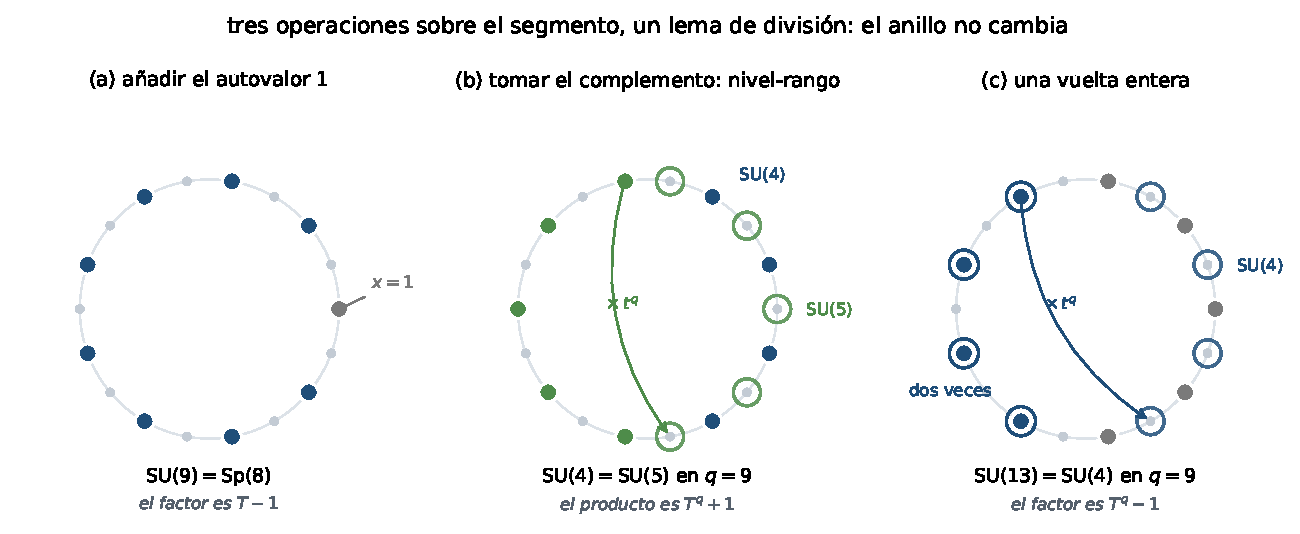
\includegraphics[width=\textwidth]{fig_operaciones_es.pdf}
\caption{Las tres operaciones de la Proposici\'on~\ref{prop:ops} sobre la circunferencia de ra\'ices
$2q$-\'esimas de la unidad, dibujadas en $q=9$. El segmento de $\SU(n)$ son $n$ exponentes
consecutivos de una clase de paridad. (a) A\~nadir el autovalor $1$ es el factor $T-1$. (b) Los $n$
exponentes y los $q-n$ restantes multiplican a $T^q+1$, y lo sobrante es el segmento de $\SU(q-n)$
girado media vuelta, que es multiplicar por $t^q=-1$; este panel es la dualidad nivel-rango, y la
media vuelta es todo lo que el lema de divisi\'on tiene que absorber. (c) Trece exponentes en $q=9$
cubren la clase una vez y cuatro de ellos dos veces; la clase completa es el factor $T^q-1$ y los
cuatro que se repiten son otra vez $\SU(4)$ salvo $t^q$.}
\label{fig:operaciones}
\end{figure}

\medido{$287$ casillas con $m\le7$, $q\le49$ para (a), comparando los dos \emph{ret\'iculos} y no
s\'olo sus \'indices; $90$ complementos y $82$ per\'iodos, tambi\'en como ret\'iculos, con $q\le21$
y $\varphi(2q)\le24$. Ninguna discrepancia.}

Dos consecuencias merecen enunciarse aparte, porque quitan un caso en vez de a\~nadirlo.

\begin{corollary}\label{cor:par}
Sea $q$ impar y $n<q$ par. Entonces $A_{\SU(n)}(q)=A_{\Sp(q-n-1)}(q)$; para $n>q$ apl\'iquese
antes la Proposici\'on~\ref{prop:ops}(c).
\end{corollary}

\begin{proof}
$q-n$ es impar, as\'i que se aplica la Proposici\'on~\ref{prop:ops}(b) y despu\'es la (a).
\end{proof}

As\'i que para $q$ impar el caso par no es una teor\'ia aparte: es el anillo de tipo $C$ en el mismo
$q$, exactamente y no s\'olo salvo conjugaci\'on. Lo que sobrevive de la \S\ref{sec:par} es el caso
$q$ par.

\begin{remark}[el segmento par es $\Sp(2m)$ en el otro elemento principal]
El segmento $\{\pm1,\pm3,\dots,\pm(2m-1)\}$ de $\SU(2m)$ es tambi\'en el segmento de $\Sp(2m)$ en
$\exp(2\pi i\rho^\vee/q)$, ya que $\rho^\vee=(m-\tfrac12,\dots,\tfrac12)$ para $C_m$ da exactamente
los exponentes impares m\'odulo $2q$. Como el espectro es cerrado por inversos, los $e_k$ de $\Sp$ y
los de $\SU(2m)$ generan el mismo anillo. Los dos elementos principales $\rho$ y $\rho^\vee$ de
$\Sp(2m)$ son, por tanto, las dos posiciones sim\'etricas de la Figura~\ref{fig:formas}, y el tipo
$A$ no a\~nade una tercera.
\end{remark}

\begin{remark}[por qu\'e ten\'ia que aparecer $\Sp$]
El par $(\SU(2m+1),\Sp(2m))$ es el plegado $A_{2m}\rightsquigarrow C_m$: el grupo fijo del
automorfismo de diagrama de $\SL(2m+1)$ es $\SO(2m+1)$, cuyo dual es $\Sp(2m)$; y $g_q$, con
espectro cerrado por inversos y determinante~$1$, est\'a salvo conjugaci\'on en ese grupo fijo. La
f\'ormula de caracteres entrelazados de Jantzen \cite{Jan,Hopper,FSS} vive en el mismo cuadro, pero
iguala un
traza \emph{torcida} con un car\'acter ordinario del dual del grupo fijo, mientras que la
Proposici\'on~\ref{prop:ops}(a) iguala valores ordinarios con valores ordinarios y se demuestra por
una divisi\'on. La citamos como contexto, no como precedente.
\end{remark}

\section{El cuadro local}\label{sec:loc}

Fijado $p$, escribamos $M=p^vq'$ con $p\nmid q'$, $E=\varphi(p^v)$, $d=\varphi(q')/2$.
Suponemos $n\not\equiv0,\pm1\pmod q$, pues en otro caso $A=\ZZ$ por la
Proposici\'on~\ref{prop:ops} y no hay nada que calcular, y $q'\ge3$: para $q'\le2$ el \'algebra
residual es $\FF_p$, $d$ debe leerse como $1$, y la matriz del Teorema~\ref{thm:loc}(b) no tiene
columnas --- en $\SU(3)$, $q=8$, $p=2$ tiene rango $0$ mientras $W_1=1$. En
$\ZZ_p[\zeta_M]$ escribamos $\zeta_M=\omega\rho$ con $\omega$ de orden $q'$ y $\rho$ de orden
$p^v$, y pongamos $\pi=\rho-1$, un uniformizante, $\gamma_c=\omega^c$, y
\[
N_c=\#\{j:a_j\equiv c\ (q')\},\qquad S(c)=\sum_{a_j\equiv c}a_j .
\]
Por la simetr\'ia del segmento, $S(-c)=-S(c)$; en particular $S(0)=0$, y $S(q'/2)=0$ cuando $q'$ es
par.

\begin{lemma}[primer orden]\label{lem:orden1}
Con $F(T)=\prod_c(T-\gamma_c)^{N_c}$,
\[
\marco{\prod_j(T-x_j)\;=\;F(T)\;-\;\pi\sum_c S(c)\,\gamma_c\,\frac{F(T)}{T-\gamma_c}\;+\;O(\pi^2).}
\]
\end{lemma}

\begin{proof}
Como $\rho=1+\pi$, cada autovalor es
$x_j=\omega^{a_j}\rho^{a_j}=\gamma_{a_j}\bigl(1+a_j\pi+O(\pi^2)\bigr)$, de modo que
$T-x_j=(T-\gamma_{a_j})-a_j\gamma_{a_j}\pi+O(\pi^2)$. Desarrollando el producto en $j$ y quedandose
con el t\'ermino lineal en $\pi$,
\[
\prod_j(T-x_j)=\prod_j(T-\gamma_{a_j})-\pi\sum_j a_j\gamma_{a_j}\prod_{i\neq j}(T-\gamma_{a_i})+O(\pi^2),
\]
y $\prod_{i\neq j}(T-\gamma_{a_i})=F(T)/(T-\gamma_{a_j})$, una divisi\'on exacta en $\cO[T]$.
Agrupar los \'indices $j$ por la clase $c=a_j\bmod q'$ convierte
$\sum_j a_j\gamma_{a_j}F(T)/(T-\gamma_{a_j})$ en $\sum_c S(c)\gamma_c F(T)/(T-\gamma_c)$.
\end{proof}

El lema dice que las partes de primer orden de \emph{todos} los generadores a la vez son los
coeficientes de un solo polinomio. No son datos independientes: en el caso estable (Definici\'on~\ref{def:est}) --- residuo escalar
y $E\ge2$, el marco de los Teoremas~\ref{thm:loc} y~\ref{thm:sombra} --- $\gr_1(A)$ es su
envolvente sobre $\FF_p$; sin estabilidad el \'algebra residual los multiplica, y en $\GL(2)$,
$q=15$, $p=3$ generan una sola direcci\'on sobre $\FF_3$ mientras la capa est\'a llena, de
dimensi\'on $4$. Est\'a
enunciado en los autovalores $x_j$, que es el modelo correcto para el anillo no real de la
\S\ref{sec:sombra}; para un segmento sim\'etrico hay que pasar antes a coordenadas reales, y de
ah\'i salen los enteros cu\'anticos de \cite{Cond}.

\begin{lemma}[coordenadas reales]\label{lem:real}
Sea el segmento sim\'etrico y escribamos $\eta_j=x_j+x_j^{-1}$, $z=(\omega-\omega^{-1})\pi$ y
\[
U_c=\frac{\omega^c-\omega^{-c}}{\omega-\omega^{-1}},
\]
el entero cu\'antico, que satisface $\sigma_u(U_c)=U_{uc}/U_u$ y se anula exactamente cuando
$2c\equiv0$. Escribamos tambi\'en $\bar\gamma_c=\gamma_c+\gamma_c^{-1}$, la contrapartida real de
$\gamma_c$, que sigue satisfaciendo $\sigma_u(\bar\gamma_c)=\bar\gamma_{uc}$. Entonces
$A=\ZZ[e_k(\eta)]$, cada $\eta_j\equiv\bar\gamma_{a_j}+a_jU_{a_j}z$ m\'odulo $\rad^2$, y
\[
\marco{\prod_j(T-\eta_j)\equiv F_\eta(T)-z\,G(T),\qquad
G(T)=\sum_c S(c)\,U_c\,\frac{F_\eta(T)}{T-\bar\gamma_c},}
\]
donde $c$ recorre un representante de cada par $\{c,-c\}$ de clases que toca el medio segmento,
tanto en la suma como en $F_\eta=\prod_c(T-\bar\gamma_c)^{N_c}$, y $N_c$ cuenta los $a_j>0$ con
$a_j\equiv\pm c$. Sumar $S(c)U_c$ sobre los dos miembros de un par contar\'ia cada t\'ermino dos
veces, pues $S(-c)=-S(c)$ y $U_{-c}=-U_c$.
\end{lemma}

\begin{proof}
Para un segmento sim\'etrico, $\prod_j(T-x_j)=(T-1)^{\varepsilon}\prod_{j>0}(T^2-\eta_jT+1)$ con
$\varepsilon\in\{0,1\}$. El factor $(T-1)^\varepsilon$ es m\'onico en $\ZZ[T]$, as\'i que por el
Lema~\ref{lem:div} puede suprimirse; y los coeficientes del producto restante son polinomios sobre
$\ZZ$ en los $e_k(\eta)$, triangularmente, y rec\'iprocamente, de modo que el anillo es
$\ZZ[e_k(\eta)]$. El desarrollo es el Lema~\ref{lem:orden1} aplicado a los $\eta_j$: de
$x_j=\gamma_{a_j}(1+a_j\pi+O(\pi^2))$,
\[
\eta_j=\gamma_{a_j}+\gamma_{a_j}^{-1}+a_j\pi(\gamma_{a_j}-\gamma_{a_j}^{-1})+O(\pi^2)
=\bar\gamma_{a_j}+a_jU_{a_j}z+O(\pi^2),
\]
y agrupar los $j>0$ por pares $\{c,-c\}$, cuyos t\'erminos $a_jU_{a_j}$ suman $S(c)U_c$, da
$G$. N\'otese que el uniformizante del anillo real es $z$ y no $\pi$ ---
salvo un t\'ermino de orden $\pi^2$: $z$ mismo no es real, pues su conjugado es $z/(1+\pi)$, y el
elemento real $z_0=\zeta_M+\zeta_M^{-1}-(\omega+\omega^{-1})$ coincide con \'el m\'odulo $\pi^2$,
que es todo lo que se usa. Los dos difieren en la unidad $\omega-\omega^{-1}$, y es exactamente esa unidad la que convierte el
coeficiente no real $\gamma_c$ del Lema~\ref{lem:orden1} en el real $U_c$. Escribir $G$ con
$\gamma_c$ en lugar de $U_c$, o con $T-\gamma_c$ en lugar de $T-\bar\gamma_c$, dar\'ia un polinomio
distinto: los dos modelos no deben mezclarse.
\end{proof}

\begin{definition}\label{def:est}
El segmento es \emph{estable} en $q'$ si el multiconjunto $\{a_j\bmod q'\}$ es invariante bajo
multiplicaci\'on por toda unidad de $\ZZ/q'$.
\end{definition}

\begin{lemma}\label{lem:est}
El segmento es estable en $q'$ si y s\'olo si $N_c$ depende \'unicamente de $\gcd(c,q')$.
\end{lemma}

\begin{proof}
Las \'orbitas de $(\ZZ/q')^\times$ sobre $\ZZ/q'$ son los conjuntos $\{c:\gcd(c,q')=D\}$, uno por
cada divisor $D$ de $q'$. Un multiconjunto es invariante exactamente cuando su funci\'on de
multiplicidad es constante sobre las \'orbitas.
\end{proof}

Escribimos $\rad$ para el radical de $\cO_p=\cO\otimes\ZZ_p$ (para el anillo real, del $\cO_p$
real), $\bar R=\cO_p/\rad$ para el \'algebra residual, de dimensi\'on $d$ sobre $\FF_p$, y
$W_i=\dim_{\FF_p}\bigl((A_p\cap\rad^i)+\rad^{i+1}\bigr)/\rad^{i+1}$ para la dimensi\'on de la capa
$i$-\'esima de $A$; $e$ es el menor $i$ con $A_p\supseteq\rad^i$, el exponente del conductor.

\begin{theorem}[estructura local; {\cite[Thm.~5]{Cond}}]\label{thm:loc}
Sup\'ongase el segmento estable en $q'$ y $E\ge2$. Entonces
\begin{enumerate}
\item[(a)] $F_\eta\in\FF_p[T]$, la imagen de $A$ en $\bar R$ es $\FF_p$ --- es decir, $W_0=1$ --- y
$A$ tiene un \'unico ideal maximal sobre $p$, con cuerpo residual $\FF_p$;
\item[(b)] $W_1=\dim_{\FF_p}\FF_p[(\ZZ/q')^\times]\cdot S$, el rango m\'odulo $p$ de
$[S(u^{-1}c)]$ con filas $u\in(\ZZ/q')^\times/\pm1$ y columnas las clases con $2c\not\equiv0$;
\item[(c)] si adem\'as $d\ge2$, entonces $e=1$ si y s\'olo si $W_1=d$;
\item[(d)] $v_p([\cO:A])=\sum_{i<e}(d-W_i)$; en particular $v_p=d-1$ cuando $e=1$ y
$v_p=2d-1-W_1$ cuando $e=2$.
\end{enumerate}
\end{theorem}

\begin{proof}
(a) La estabilidad hace que el grupo de Galois permute los factores de $F_\eta$, as\'i que sus
coeficientes quedan fijos y $F_\eta\in\FF_p[T]$; los $e_k$ se reducen a esas constantes en todo
cuerpo residual.

(b) Todo elemento de $A$ es $\Phi(e)$ con $\Phi\in\ZZ[X]$, y m\'odulo $\rad^2$,
\[
\Phi(e)\;\equiv\;\Phi(F_\eta)+z\sum_k(\partial_k\Phi)(F_\eta)\,G_k ,
\]
con $\Phi(F_\eta)\in\FF_p$ y $p\in\rad^2$ porque $E\ge2$. As\'i que $\gr_1(A)$ es la envolvente
sobre $\FF_p$, $V$, de los coeficientes $G_k$, que por el Lema~\ref{lem:real} son los de $G$. Como
$\bar R$ es \'etale, $\bar R\otimes\overline{\FF}_p\cong\overline{\FF}_p^{\,d}$ a trav\'es de las
inmersiones $\sigma_u$, y la extensi\'on de escalares es inyectiva sobre subespacios de $\FF_p$, de
modo que $\dim V$ es el rango de la matriz cuya fila $u$ lista los coeficientes de $\sigma_u(G)$. De
$\sigma_u(\bar\gamma_c)=\bar\gamma_{uc}$, $\sigma_u(U_c)=U_{uc}/U_u$ y la estabilidad de $F_\eta$,
\[
U_u\,\sigma_u(G)=\sum_c S(u^{-1}c)\,U_c\,\frac{F_\eta(T)}{T-\bar\gamma_c},
\]
y multiplicar una fila por la unidad $U_u$ no cambia el rango; las funciones
$U_cF_\eta/(T-\bar\gamma_c)$, una por cada clase $c$ salvo signo, son independientes y no
dependen de $u$ --- las clases $c$ y $-c$ dan funciones opuestas y columnas que coinciden salvo
signo, as\'i que conservar las dos no cambia el rango --- y las clases con $2c\equiv0$ no aportan
nada porque all\'i $U_c=0$ (y $S(c)=0$).

(c) Si $\gr_1(A)=\gr_1(\cO)$ entonces $\gr_i(A)\supseteq\gr_1(A)^i=\gr_i(\cO)$ para todo $i$, ya que
$\gr(\cO_p)$ es un anillo de polinomios sobre $\bar R$, y la filtraci\'on colapsa, luego $e\le1$; y
$e\ge1$ porque $W_0=1<d$ hace $A_p\ne\cO_p$. El rec\'iproco es claro.

(d) Fil\'trense $\cO_p$ y $A_p$ por $\rad^i$; para $i\ge e$ se tiene $A_p\cap\rad^i=\rad^i$, as\'i
que s\'olo contribuyen las capas $i<e$, con cocientes de dimensi\'on $d-W_i$. La capa $i=0$
contribuye siempre $d-1$, por (a).
\end{proof}

\medido{El instrumento reproduce la ley publicada de tipo $C$ en $18$ de $18$ casillas. En tipo $A$,
(d) con $e=2$ vale en $44$ de $44$ casillas bajo $W_1>d/2$; de las $18$ casillas fuera de la
hip\'otesis, $15$ siguen coincidiendo y las $3$ que fallan tienen todas $W_1=0$, la zona de la
escalera de \cite{Cond}. El
enunciado (b) vale en $193$ de $193$ casillas estables y en $98$ de $127$ inestables: la
hip\'otesis no es decoraci\'on. Que $W_0=1$ no se supone, sino que se lee en el instrumento en cada
casilla tabulada en la \S\ref{sec:sop}.}

La \'ultima cl\'ausula de (d) merece decirse en voz alta, porque es sobre lo que se apoya la
\S\ref{sec:sop}: bajo las hip\'otesis del teorema el defecto no es nunca cero en cuanto $d\ge2$. Una
primera capa llena hace $e=1$, no $v_p=0$.

Que $d\ge2$ tampoco es decoraci\'on, y por eso lo lleva (c) mientras las otras tres partes no. En
$\SU(3)$ con $q=12$ y $p=3$ el segmento $\{1,0,-1\}$ es estable en $q'=4$ con $E=2$, y $d=1$, as\'i
que $W_1=1=d$ --- y sin embargo $A=\ZZ[\sqrt3]=\cO$ es maximal, $\mathfrak f=\cO$ y $e=0$. Lo que
falla no es el recuento de capas sino el paso anterior: $W_0=1$ deja de forzar un defecto en cuanto
$d=1$, y entonces $e=1$ no tiene a qu\'e referirse. Las partes (a), (b) y (d) aguantan tal cual, y
(d) se lee como la suma vac\'ia. La fuente deja fuera esa misma esquina excluyendo
$q'\in\{1,2,3,4,6\}$ entre sus hip\'otesis permanentes \cite[\S5]{Cond}.

El enunciado (d) es un plano, y merece verse como tal. Sobre un barrido m\'as amplio de $417$
casillas, el anillo real vive con $d=\varphi(q')/2$ y la sombra de la \S\ref{sec:sombra} con
$D=\varphi(q')$; si se pone la dimensi\'on de la capa en un eje, \emph{las dos} poblaciones caen en
el mismo plano $v=2\dim-1-W_1$. \'Esa es la tesis de esta nota en una imagen: el grupo no entra,
s\'olo entra el segmento.

El plano es la cara $e=2$ de (d), y conviene saber qu\'e hay fuera de ella. En el r\'egimen del
Teorema~\ref{obs:puente} con $p\nmid N$ y el perfil real de \cite{Cond} (la f\'ormula que sigue a la
Proposici\'on~\ref{prop:tau}), escribiendo $\delta=d-W_1(R)$ para la ca\'ida de la primera capa real,
la sombra tiene $W_1=d+1-\delta$ y $\dim=2d$, de modo que el plano
predecir\'ia $3d-2+\delta$ mientras que el \'indice verdadero es $3d-2+2\delta$: una casilla de la
sombra queda \emph{exactamente $\delta$ por encima del plano}, y la altura sobre el plano es el
defecto del n\'umero de clases. Con $p\mid N$ la cuenta es otra: en $q=45$, $p=3$, $N=3$ la sombra
tiene $W_1=0$ y $v_3([\cO:B])=14$, donde esta lectura dar\'ia $1$ y $8$. Ninguna casilla del barrido lo muestra --- sus $14$ casillas de
sombra fuera del plano tienen todas $p=2$ o $(p,q')=(3,4)$, fuera de ese r\'egimen, y el barrido
nunca llega al primer conductor con $\delta>0$ --- as\'i que la figura es una imagen de la cara
$\delta=0$.

\begin{figure}[htbp]
\centering
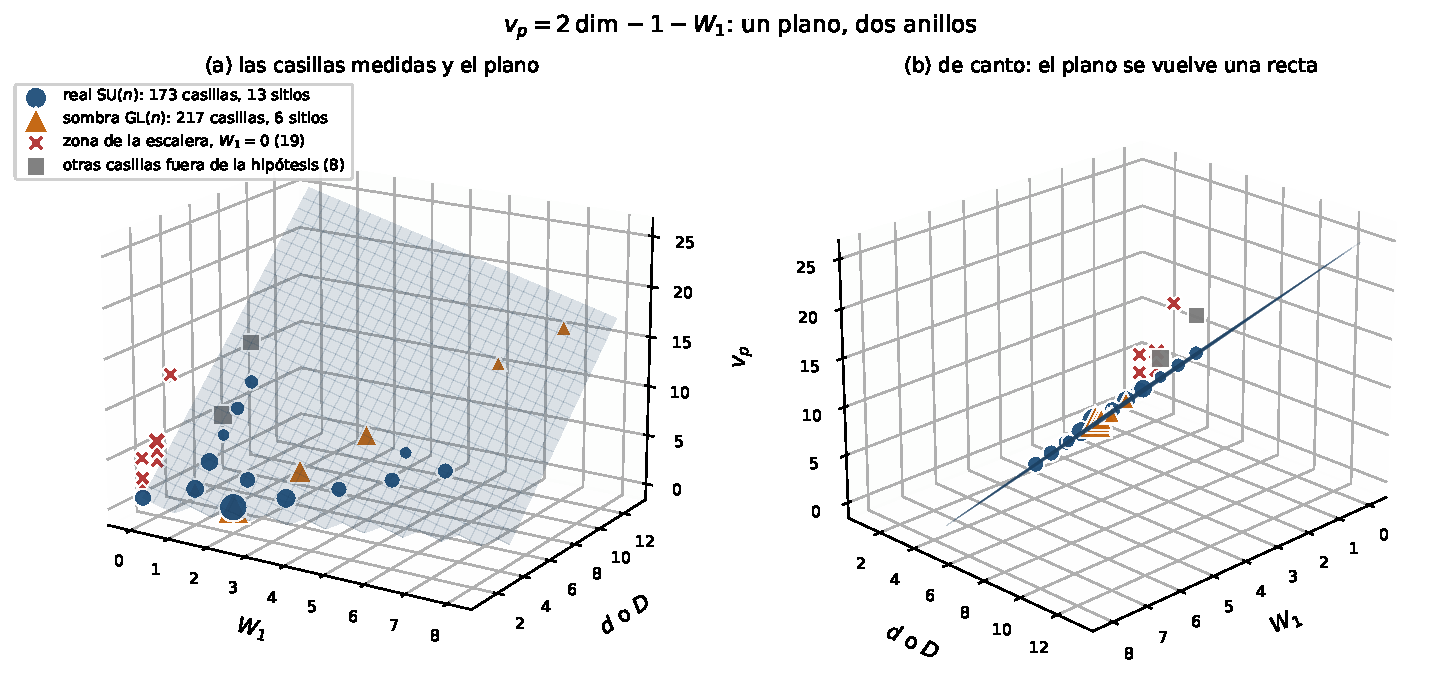
\includegraphics[width=\textwidth]{fig_plano_es.pdf}
\caption{Cada casilla medida es un punto $(W_1,\dim,v_p)$; muchas casillas comparten posici\'on, y
el tama\~no del marcador dice cu\'antas. \emph{Izquierda}: las casillas y el plano.
\emph{Derecha}: visto a lo largo de $(1,1,1)$, que es ortogonal a la normal $(1,-2,1)$, el plano se
proyecta en una recta y todo lo que est\'a sobre \'el se vuelve colineal. Bajo la hip\'otesis
$W_1>\dim/2$ las $335$ casillas caen en el plano; las $27$ que no, se muestran aparte, $19$ de ellas
en la zona de la escalera $W_1=0$. Las $14$ casillas de sombra fuera del plano tienen todas $p=2$ o
$(p,q')=(3,4)$; ninguna est\'a en el r\'egimen del Teorema~\ref{obs:puente}, donde la sombra se
separa del plano hacia arriba exactamente en $\delta$.}
\label{fig:plano}
\end{figure}

\section{Soporte: qu\'e primos pueden aparecer}\label{sec:sop}

A lo largo de esta secci\'on escribimos
\[
r=\frac{q}{p^{v_p(q)}},
\]
la parte prima con $p$ de $q$ --- no de $M$. Para $n$ impar, y para $n$ par con $p=2$, se tiene
$r=q'$. Para $n$ par y $p$ impar, $M=2q$ da $q'=2r$: el segmento ocupa entonces los residuos
impares m\'odulo $2r$, que como progresi\'on aritm\'etica tiene per\'iodo $r$, y $r$ es el m\'odulo
que ve el criterio.

\begin{proposition}\label{prop:fam}
Si $r$ divide a $n-1$, $n$ o $n+1$, entonces el segmento de $\SU(n)$ es estable en $q'$.
\end{proposition}

\begin{proof}
Por el Lema~\ref{lem:est} basta ver que $N$ es constante sobre las \'orbitas de $(\ZZ/q')^\times$.
Hay tres ramas. Para $n$ impar, $M=q$ y $q'=r$, y el segmento $\{-m,\dots,m\}$ son $n$ residuos
consecutivos de $\ZZ/r$. Para $n$ par es la progresi\'on $\pm1,\pm3,\dots,\pm(n-1)$ de diferencia
$2$ m\'odulo $M=2q$: con $p=2$ se tiene $q'=r$ impar y la diferencia es invertible, y con $p$ impar
se tiene $q'=2r$ y la progresi\'on recorre las clases impares, volviendo al principio tras $r$
pasos. En toda rama la progresi\'on tiene per\'iodo $r$, as\'i que las clases que no encuentra son
o ninguna o todas las pares, y \'esas las permutan entre s\'i las unidades, as\'i que no aportan
nada. En las clases que s\'i encuentra, $N_c\in\{\lfloor n/r\rfloor,\lceil n/r\rceil\}$, y los dos
valores coinciden cuando $r\mid n$. Si $n\equiv\pm1\pmod r$, exactamente una clase $c$ se desv\'ia
en uno, y como el segmento es sim\'etrico $N_{-c}=N_c$, de modo que esa clase cumple $c\equiv-c$.
Una clase as\'i queda fija por toda unidad, porque la \'orbita de $c$ tiene
$\varphi(q'/\gcd(c,q'))$ elementos y eso es $1$ exactamente cuando $2c\equiv0$. Luego $N$ es
constante sobre las \'orbitas. (Para $n$ impar la clase excepcional no es siempre el centro $0$:
escribiendo $n=Ar\pm1$ es $Ar/2\bmod r$, que es $q'/2$ cuando $A$ es impar --- en $\SU(5)$ con
$q'=4$ es $2$.)
\end{proof}

\medido{$807$ casillas con $n\le25$, $q\le60$, sobre las cuatro ramas (las dos paridades de $n$ y
de $r$): toda casilla de una familia es estable, sin excepci\'on.}

El rec\'iproco falla: hay segmentos estables fuera de las familias, el menor $n=3$, $q'=6$, cuyos
residuos $\{0,1,5\}$ son la uni\'on de las \'orbitas $\{0\}$ y $\{1,5\}$. Todos ellos tienen
$q'=6$, como obligar\'a el Lema~\ref{lem:inter}, y son maximales por la raz\'on dada en la
demostraci\'on de la Proposici\'on~\ref{prop:sop}: all\'i $d=1$ y $W_1=1$. No es $d=1$ por s\'i
solo: dentro de las familias, $d=1$ puede llevar un defecto.

Dentro de las familias el defecto no es meramente posible: est\'a forzado, y por la propia ley
local.

\begin{proposition}[las familias dan siempre defecto]\label{prop:conv}
Sea $E\ge2$, sea el segmento estable en $q'$ --- por la Proposici\'on~\ref{prop:fam} basta con que
$r$ divida a uno de $n-1,n,n+1$ --- y sea $\varphi(q')\ge4$, es decir $q'\notin\{1,2,3,4,6\}$, es
decir $d\ge2$. Entonces
\[
\marco{p\mid[\cO:A],\qquad\text{y de hecho } v_p([\cO:A])\ \ge\ d-1 .}
\]
\end{proposition}

\begin{proof}
Se aplica el Teorema~\ref{thm:loc}. Por (a) la capa $i=0$ aporta $d-W_0=d-1$ a la suma de (d), y
todo t\'ermino de esa suma es $\ge0$.
\end{proof}

As\'i que dentro de las familias un defecto s\'olo puede evitarse en el rango $\varphi(q')\le2$,
donde $d=1$ y el argumento no dice nada: la capa $i=0$ est\'a entonces llena sin m\'as, y un
defecto, si lo hay, est\'a en las capas m\'as profundas. Puede haberlo: $\SU(11)$ en $q=36$ y $p=3$
est\'a en la familia $r=4\mid12$, tiene $d=1$, y tiene \'indice $3$, con perfil $(1,0,1,\dots)$.

\medido{$26$ de $26$ casillas estables con $E\ge2$ y $d\ge2$, sobre $n\le7$ y $q\le40$, cumplen
$v_p\ge d-1$; restringiendo a las casillas de una familia con $r\notin\{1,2,3,4,6\}$, $23$ de $23$
cumplen $p\mid[\cO:A]$.}

\begin{lemma}[intervalos estables]\label{lem:inter}
Sea $q'\ge3$ y sea $I\subseteq\ZZ/q'$ un conjunto de $B$ residuos consecutivos con
$2\le B\le q'-2$. Si $\alpha(I)=I$ para una biyecci\'on af\'in $\alpha(x)=ux+b$ de $\ZZ/q'$,
entonces $u\equiv\pm1\pmod{q'}$. En particular, si
$I$ es uni\'on de los estratos $X_D=\{c:\gcd(c,q')=D\}$ entonces $\varphi(q')\le2$; de hecho los
\'unicos $I$ as\'i aparecen en $q'=6$, $B=3$, y son $\{5,0,1\}=X_1\cup X_6$ y
$\{2,3,4\}=X_2\cup X_3$.
\end{lemma}

\begin{proof}
El complemento de un intervalo c\'iclico propio es un intervalo c\'iclico, y es $\alpha$-estable
si $I$ lo es; as\'i que podemos sustituir $I$ por el m\'as corto de los dos, un intervalo $J$ de
longitud $b$ con $2\le b\le q'/2$ y $\alpha(J)=J$. P\'ongase $C_J(t)=|J\cap(J+t)|$. La biyecci\'on
$\alpha$ lleva $J\cap(J+t)$ sobre $\alpha(J)\cap(\alpha(J)+ut)=J\cap(J+ut)$, luego
$C_J(ut)=C_J(t)$, y en
particular $C_J(u)=C_J(1)=b-1$. Por otro lado $C_J$ no cambia al trasladar $J$, y para
$J=\{0,\dots,b-1\}$ y $1\le t<q'$
\[
C_J(t)=\max(0,b-t)+\max(0,b-(q'-t)).
\]
Como $2b\le q'$ los dos sumandos nunca son positivos a la vez, y $b-1\ge1$; as\'i que $C_J(t)=b-1$
exactamente cuando $t=1$ o $t=q'-1$, y $u\equiv\pm1$.

Si $I$ es uni\'on de estratos es estable por toda unidad, porque multiplicar por una unidad no
cambia $\gcd(c,q')$. Luego toda unidad es $\pm1$, es decir $\varphi(q')\le2$ y $q'\in\{3,4,6\}$. En
$q'=3$ el rango de $B$ es vac\'io. Escribiendo $I=\{a,\dots,a+B-1\}$, la estabilidad por $-1$ se lee
$2a+B-1\equiv0\pmod{q'}$, que con $q'$ par obliga a $B$ impar: eso excluye $q'=4$, donde $B=2$, y
deja $q'=6$, $B=3$, $a\in\{2,5\}$.
\end{proof}

\medido{La forma fuerte por fuerza bruta: para todo $q'\le120$, todo intervalo con
$2\le B\le q'-2$ y toda unidad $u$, $uI=I$ s\'olo para $u=\pm1$ ($3{,}1\times10^7$ comprobaciones),
y la forma af\'in para $q'\le60$ y toda traslaci\'on $b$ ($1{,}9\times10^6$ comprobaciones); y sobre
todos los $q'\le150$, todos los $B$ y todas las rotaciones, el \'unico intervalo que es
uni\'on de estratos fuera de $B\in\{0,1,q'-1\}$ es uno de los dos de $q'=6$. La cota $B\ge2$ no es
decoraci\'on: el conjunto $\{0\}$ es estable por toda unidad. Es el mismo $q'=6$ de las casillas
registradas m\'as abajo.}

\begin{proposition}[soporte]\label{prop:sop}
Sup\'ongase que $r$ no divide a ninguno de $n-1$, $n$, $n+1$. Entonces, o bien el segmento es
estable en $q'$, y entonces $q'=r=6$ y $A$ es maximal en $p$; o bien no lo es, y entonces la imagen
de $A$ en $\bar R$ es todo $\bar R$, es decir $W_0=d$, y $A$ es maximal en $p$ cuando $v=0$.
\end{proposition}

\begin{proof}
Sup\'ongase que $r$ no divide a ninguno de los tres. Como en la demostraci\'on de la
Proposici\'on~\ref{prop:fam}, escr\'ibase el segmento en orden como $a_j=a_0+\beta j$, $0\le j<n$,
con $\beta=1$ para $n$ impar y $\beta=2$ para $n$ par; la clase de $a_j$ m\'odulo $q'$ depende de
$j$ s\'olo m\'odulo $r$. Escribiendo $n=Ar+B$, la multiplicidad vale $A+1$ en las clases de las
posiciones $J=\{0,\dots,B-1\}\subseteq\ZZ/r$ y $A$ en las dem\'as, y $B\notin\{0,1,r-1\}$, as\'i
que $2\le B\le r-2$. Una unidad $u$ de $\ZZ/q'$ env\'ia $a_j$ a
$a_0+\beta\bigl(uj+(u-1)a_0/\beta\bigr)$ --- para $\beta=2$ el n\'umero $a_0$ es impar y $u$ es
impar ---, as\'i que sobre las posiciones act\'ua como la biyecci\'on af\'in
$\alpha_u(j)=uj+(u-1)a_0/\beta$ de $\ZZ/r$. La aplicaci\'on $u\mapsto\alpha_u$ es inyectiva: $u$
queda determinada por $u\bmod r$ salvo si $q'=2r$ con $r$ par, y entonces $u$ y $u+r$ difieren en
la traslaci\'on $r/2$.

Si $v=0$ el primo es no ramificado y $\cO_p/p\cO_p=\bar R$, as\'i que los dos casos de abajo, que
terminan con una imagen residual llena, dan $A_p=\cO_p$ por Nakayama sin frontera alguna.
Sup\'ongase el segmento estable en $q'$. Entonces $\alpha_u(J)=J$ para toda unidad, y el
Lema~\ref{lem:inter} da $u\equiv\pm1\pmod r$. Una aplicaci\'on af\'in de parte lineal $1$ fija el
intervalo propio $J$ s\'olo si es la identidad, ya que $C_J(t)<C_J(0)$ para $t\ne0$, y una de parte
lineal $-1$ queda entonces determinada por $J$; as\'i que las unidades dan a lo sumo dos
aplicaciones, y $\varphi(q')\le2$. Con $r\ge4$, obligado por $2\le B\le r-2$, y $q'\in\{r,2r\}$
esto deja $q'=r\in\{4,6\}$; $q'=r$ par significa $n$ impar, y en $r=4$ eso obliga a $B$ impar,
fuera de $[2,2]$. As\'i que $q'=r=6$, luego $n$ es impar, $B=3$ y $n=6A+3$; y $p\ge5$, as\'i que
$E\ge4$ cuando $v\ge1$. All\'i $d=1$ y la imagen residual es todo $\bar R=\FF_p$, lo que zanja
$v=0$. Para $v\ge1$ el anillo residual $\bar R$ es $\FF_p$, y $\cO_p$ es un anillo de valoraci\'on
discreta totalmente ramificado sobre $\ZZ_p$: est\'a generado sobre $\ZZ_p$ por cualquier elemento
de valoraci\'on uno, as\'i que $A_p=\cO_p$ en cuanto $W_1=1$. Por el Teorema~\ref{thm:loc}(b),
$W_1$ es el rango de la \'unica fila $(S(1),S(2),-S(2),-S(1))$ sobre las clases $1,2,4,5$, y sumar
sobre $\{-m,\dots,m\}$ da $(S(1),S(2))=(A+1,-A)$ para $A$ par y $(A,-(A+1))$ para $A$ impar. Dos
enteros consecutivos no son ambos divisibles por $p$; as\'i que $W_1=1$ y no hay defecto.

En otro caso el segmento es inestable en $q'$, y vale m\'as: por los mismos dos pasos una unidad
que fija el multiconjunto da una $\alpha_u$ que fija $J$, luego $u\equiv\pm1$ y $\alpha_u$ es una
de a lo sumo dos aplicaciones, as\'i que el estabilizador del multiconjunto en
$(\ZZ/q')^\times/\pm1$ es trivial. Entonces la imagen de $A$ en $\bar R$ es todo $\bar R$, es
decir $W_0=d$: esa imagen est\'a generada por los coeficientes de $F_\eta$, y tras extender
escalares $\bar R\otimes\overline\FF_p\cong\overline\FF_p^{\,d}$ a trav\'es de las inmersiones
$\sigma_u$, un coeficiente se convierte en la funci\'on $u\mapsto$ (ese coeficiente de
$\sigma_u(F_\eta)$). Como los $\bar\gamma_c$ son distintos para clases $c\not\equiv\pm c'$, dos
inmersiones dan el mismo polinomio s\'olo si $u'u^{-1}$ fija el multiconjunto, as\'i que esas
funciones separan los $d$ puntos, y funciones que separan los puntos de un conjunto finito generan
todas las funciones sobre \'el.
\end{proof}

Una imagen residual llena no hace por s\'i sola maximal al orden: la ley del \'indice del
Teorema~\ref{thm:loc} dice $v_p([\cO:A])=\sum_{i<e}(d-W_i)$, y $W_0=d$ mata el t\'ermino $i=0$ y
ning\'un otro. Lo que cierra el hueco es que, una vez alcanzado el cuerpo residual, la primera capa
lo decide todo, y la primera capa se lee en los momentos.

\begin{proposition}[la primera capa decide]\label{prop:tangente}
Sea $E\ge2$ y sup\'ongase que la imagen de $A$ en $\bar R$ es todo $\bar R$. Entonces $A_p=\cO_p$ si
y s\'olo si $p\nmid S(c)$ para alguna clase $c$, tomada con $2c\not\equiv0$ cuando el segmento es
sim\'etrico.
\end{proposition}

\begin{proof}
El anillo graduado $\gr(A)$ es un subanillo graduado de $\gr(\cO_p)=\bar R[\bar\varpi]$, polinomial
en la clase de un uniformizante, y $\gr_0(A)=\bar R$ por hip\'otesis. As\'i $\gr_1(A)$ es un
$\bar R$-subm\'odulo de $\gr_1(\cO_p)=\bar R\,\bar\varpi$ y $\gr_i(A)\supseteq\gr_1(A)^i$: si
$\gr_1(A)=\gr_1(\cO_p)$ todas las capas est\'an llenas y $A_p=\cO_p$, y rec\'iprocamente un orden
maximal tiene $W_1=d$. Queda identificar $\gr_1(A)$. Cada generador es
$e_k=e_k^{(0)}+g_k\varpi+O(\varpi^2)$, con $e_k^{(0)}$ el coeficiente correspondiente de $F$ (o de
$F_\eta$), que vive en el subanillo no ramificado $\ZZ_p[\omega]$, y $g_k$ el coeficiente
correspondiente de $G$ en el Lema~\ref{lem:orden1} (o en el Lema~\ref{lem:real}). Un elemento
$\Phi(e)$, $\Phi\in\ZZ_p[X]$, est\'a en $\rad$ exactamente cuando $\Phi(\bar e)=0$ en $\bar R$;
entonces $\Phi(e^{(0)})\in\rad\cap\ZZ_p[\omega]=p\,\ZZ_p[\omega]\subseteq\rad^E\subseteq\rad^2$, as\'i
que la imagen de $\Phi(e)$ en $\gr_1$ es $\sum_k(\partial_k\Phi)(\bar e)\,g_k$. Como $\bar R$ es
\'etale sobre $\FF_p$, los vectores $\bigl((\partial_k\Phi)(\bar e)\bigr)_k$ con $\Phi(\bar e)=0$
generan $\bar R^{\,n}$ --- para $\bar R=\FF_p[X]/I$ la sucesi\'on conormal da
$I/I^2\cong\bar R^{\,n}$, porque $\Omega_{\bar R/\FF_p}=0$. As\'i $\gr_1(A)$ es el $\bar R$-span de
los coeficientes de $G$, y es todo $\gr_1(\cO_p)$ exactamente cuando $G$ no se anula en ning\'un
factor de $\bar R$. En cada factor, cancelando $F$ (o $F_\eta$) en el cuerpo de funciones racionales,
las fracciones $1/(T-\gamma_c)$ de clases distintas son independientes, y $\gamma_c$ y $U_c$
($2c\not\equiv0$) son unidades; as\'i $G$ no se anula en un factor exactamente cuando alg\'un $S(c)$ es
primo con $p$, condici\'on que no depende del factor.
\end{proof}

\begin{theorem}[soporte]\label{thm:sop}
Sea $2\le n\le q-2$. Si $p$ divide a $[\cO:A]$, entonces $r$ divide a $n-1$, $n$ o $n+1$. Vale para
todo primo $p$, incluido $p=2$.
\end{theorem}

\begin{proof}
Sup\'ongase que $r$ no divide a ninguno de los tres. Por la Proposici\'on~\ref{prop:sop}, o bien
$q'=r=6$ y $A$ es maximal en $p$, o bien la imagen residual es llena. En el segundo caso, si $E=1$
la extensi\'on es no ramificada y Nakayama da $A_p=\cO_p$; si $E\ge2$, la
Proposici\'on~\ref{prop:tangente} pide una clase con $p\nmid S(c)$. Mant\'engase la notaci\'on de la
demostraci\'on de la Proposici\'on~\ref{prop:sop}: $a_j=a_0+\beta j$, $n=Ar+B$ con $2\le B\le r-2$,
la clase de $a_j$ depende s\'olo de $j\bmod r$ y lo hace biyectivamente sobre las clases que toca el
segmento, con multiplicidad $m_i=A+1$ en las posiciones $i<B$ y $A$ en las dem\'as. Sumando cada
progresi\'on,
\[
S_i=m_i(a_0+\beta i)+\beta r\,\frac{m_i(m_i-1)}2,\qquad\text{as\'i que}\qquad S_{i+1}-S_i=m\beta
\]
siempre que las posiciones $i$ e $i+1$ lleven la misma multiplicidad $m$; los pares $(0,1)$ y
$(B,B+1)$ son pares as\'i, uno en cada bloque. Si $p$ dividiera a todos los $S(c)$ --- incluidas las
clases con $2c\equiv0$, donde un segmento sim\'etrico tiene $S(c)=0$ de todos modos --- y $p\nmid\beta$,
dividir\'ia a $(A+1)\beta$ y a $A\beta$, luego a $A+1$ y a $A$. Ahora $\beta\in\{1,2\}$, as\'i que
$p\nmid\beta$ salvo si $p=2$ y $n$ es par; y entonces todo exponente es impar, $S(c)\equiv N_c\pmod2$,
y las dos multiplicidades $A$ y $A+1$ aparecen ambas, con paridades opuestas. En cualquier caso
alg\'un $S(c)$ es primo con $p$.
\end{proof}

\noindent As\'i la Proposici\'on~\ref{prop:conv} y el Teorema~\ref{thm:sop} dicen juntos que, cuando
$E\ge2$ y $\varphi(q')\ge4$, el primo $p$ divide al \'indice exactamente en las tres familias. Lo
deciden dos pasos, y son de clases distintas: el Lema~\ref{lem:inter} es un recuento, cu\'anto se
solapa un intervalo con sus trasladados, y llena la imagen residual; despu\'es los momentos llenan la
primera capa. En el caso estable la primera capa no puede hacerlo --- por el
Teorema~\ref{thm:loc}(d) una primera capa llena da $e=1$ y $v_p=d-1>0$ ---, y por eso el lema tiene
que ir primero. En coherencia con ello, las $8$ casillas estables fuera de las familias con
$n\le25$, $q\le60$ tienen todas $q'=6$, el \'unico valor que el lema permite.

\medido{De $7714$ casillas fuera de las familias con $n\le60$ y $q\le150$, las $80$ que son estables
tienen todas $n$ impar y $q'=r=6$, y las $26$ de ellas al alcance del instrumento son maximales;
$195$ casillas, $39$ de ellas con \'indice $>1$, y ning\'un primo fuera de las familias. La
Proposici\'on~\ref{prop:tangente} frente al \'indice sumado sobre todas las capas: $3060$ de $3060$
casillas con $W_0=d$, $q\le60$, $p$ impar, $E\ge2$, para $\SU(n)$, $\GL(n)$ y $\Sp(2m)$. Y sobre
$147\,926$ segmentos inestables fuera de las familias con $q\le400$ y $p$ impar, ninguno tiene todos
sus momentos divisibles por $p$.}

El mismo recuento resuelve el anillo no real de la \S\ref{sec:sombra}, y all\'i el soporte es m\'as
estrecho.

\begin{corollary}[soporte de la sombra]\label{cor:sopsombra}
Para el anillo $B_n(q)$ de la \S\ref{sec:sombra} con $2\le n\le q-2$: si $p$ divide a
$[\cO:B_n(q)]$, entonces $r$ divide a $n$ o a $n-1$.
\end{corollary}

\begin{proof}
Aqu\'i $a_j=j$, $\beta=1$ y $q'=r$. Sup\'ongase que $r$ no divide ni a $n$ ni a $n-1$, de modo que
$B=n\bmod r$ est\'a en $[2,r-1]$. Una unidad que fija el multiconjunto de clases fija las posiciones
de multiplicidad mayor, $J=\{0,\dots,B-1\}$: para $B\le r-2$ el Lema~\ref{lem:inter} deja $u=\pm1$,
y $u=-1$ lleva $1\in J$ a $r-1\notin J$; para $B=r-1$ fija la \'unica clase de multiplicidad menor,
$r-1$, as\'i que $u=1$. El estabilizador es trivial, la imagen residual es llena por el argumento de
la Proposici\'on~\ref{prop:sop}, y se aplica Nakayama ($E=1$) o la Proposici\'on~\ref{prop:tangente}
($E\ge2$). Para $B\le r-2$ concluyen los dos pares de la demostraci\'on del Teorema~\ref{thm:sop}.
Para $B=r-1$ el par $(0,1)$ da $p\mid A+1$, y entonces
$S_0+S_{r-1}=A(r-1)+rA^2=A(r-1+rA)\equiv1\pmod p$, as\'i que no se anulan los dos.
\end{proof}

\medido{El Corolario~\ref{cor:sopsombra} en la \'unica familia que excluye y el
Teorema~\ref{thm:sop} admite, $r\mid n+1$: $543$ casillas con $q\le90$, ning\'un defecto.}

\section{Los dos reg\'imenes pares}\label{sec:par}

Para $q$ impar, el Corolario~\ref{cor:par} ya ha despachado el caso $n$ par: el anillo es un anillo
de tipo $C$ en el mismo $q$. Lo que sigue es el caso restante, $q$ par, donde el complemento
mantiene $n$ par y hay que decir algo. El primo lo parte en dos: si $p=2$ entonces $v_2(M)=v_2(q)+1$
y $q'$ es impar, as\'i que $2$ es una unidad; si $p$ es impar entonces $q'=2r$ es par y $2$ no lo
es.

\begin{proposition}\label{prop:par2}
Sea $n=2m$ y sea $q'$ impar. Entonces la multiplicaci\'on por $2^{-1}$ lleva el segmento
$\{\pm1,\pm3,\dots,\pm(2m-1)\}$ sobre el bloque de $n$ residuos consecutivos centrado en $q'/2$.
\end{proposition}

\begin{proof}
Como $2\bigl(i-\tfrac{q'+1}{2}\bigr)=2i-(q'+1)\equiv2i-1$, se tiene
$2^{-1}(2i-1)\equiv i-\tfrac{q'+1}{2}$. Cuando $i$ recorre de $1$ a $m$ \'estos son los $m$ residuos
consecutivos $\tfrac{q'+1}{2}-m,\dots,\tfrac{q'+1}{2}-1$ salvo signo, y sus opuestos son
$\tfrac{q'+1}{2},\dots,\tfrac{q'+1}{2}+m-1$. La uni\'on es el bloque de $2m=n$ residuos
consecutivos de $\tfrac{q'+1}{2}-m$ a $\tfrac{q'+1}{2}+m-1$, cuyo centro es
$\tfrac{q'+1}{2}-\tfrac12=q'/2$.
\end{proof}

Multiplicar por una unidad es un automorfismo de Galois, as\'i que permuta las clases de
residuos; pero no permuta con ellas los pesos enteros $S(c)$ del Teorema~\ref{thm:loc}(b), y el
rango puede cambiar --- en $\SU(4)$, $q=20$, $p=2$, $q'=5$ los momentos del segmento son
$(0,1,-3,3,-1)$, de rango $1$ m\'odulo $2$, mientras que el diente de sierra desplazado
$(0,1,2,-2,-1)$ tiene rango $2$. As\'i que la proposici\'on es un enunciado sobre clases. N\'otese
la diferencia de fuerza entre esto y el Corolario~\ref{cor:par}: un automorfismo de Galois preserva
el rango y el \'indice de aquello a lo que se aplica, el complemento preserva el anillo mismo.

Los pesos, sin embargo, pueden calcularse directamente. Escr\'ibase $\widehat s_f$ para el diente
de sierra desplazado de per\'iodo $f$: $\widehat s_f(0)=\widehat s_f(f/2)=0$, $\widehat s_f(c)=c$
para $0<c<f/2$ y $c-f$ para $f/2<c<f$.

\begin{proposition}[la primera capa en el r\'egimen par]\label{prop:parimp}
Sean $p$ impar, $v\ge1$, $r\ge2$ par con $p\nmid r$, $q=p^vr$, y $n=Nr$ con $1\le N<p^v$ --- la
\'unica familia estable con $n$ par. Entonces $W_1=0$ si $p\mid N$, y en otro caso $W_1$ es el rango
m\'odulo $p$ de $\bigl[\widehat s_{2r}(u^{-1}c)\bigr]$, con filas $u\in(\ZZ/2r)^\times/\pm1$ y
columnas las clases \emph{impares} $c$.
\end{proposition}

\begin{proof}
Aqu\'i $M=2q$, $q'=2r$, y los exponentes $a_j=n-1-2j$ son impares. La clase $c$ que toca la
posici\'on $i$ recibe los $N$ exponentes $n-1-2i-2tr$, $0\le t<N$, cuya suma es $N(r-1-2i)$; y
$c\equiv Nr-1-2i\pmod{2r}$. Para $N$ impar esto dice $S(c)=N\,\widehat s_{2r}(c)$; para $N$ par,
$S(c)=N(c-r)=N\,\widehat s_{2r}\bigl((1+r)c\bigr)$, y $1+r$ es una unidad m\'odulo $2r$, as\'i que
s\'olo permuta las columnas. Las clases pares no se tocan. El Teorema~\ref{thm:loc}(b) da ahora el
rango, y $N$ es una unidad salvo si $p\mid N$, donde todo $S(c)$ se anula.
\end{proof}

\noindent Lo que \emph{no} se sigue es la identificaci\'on con la matriz completa de medio per\'iodo
de \cite{Cond}. Con todas las columnas, $\widehat s_f(c)=\tfrac12 s_f(c+f/2)$ y una traslaci\'on
conmuta con las unidades, as\'i que la matriz desplazada completa tiene el rango de la ordinaria; pero
la proposici\'on s\'olo conserva las columnas impares, y esa restricci\'on puede perder rango. En
$\SU(14)$, $q=70$, $p=5$ --- as\'i $r=14$, $N=1$, y $5\nmid\varphi(28)$ --- las columnas impares
tienen rango $5$ y todas las columnas rango $6$; el instrumento devuelve $W=(1,5,6,6,\dots)$ y
$v_5([\cO:A])=6$. La p\'erdida no es un efecto de escalera ni un fallo de semisimplicidad.

\begin{proposition}\label{prop:par1}
Sea $n$ par, $p$ impar y $q'=2r$ con $r$ impar. Entonces $M_{2r}$ y $M_r$ tienen el mismo rango
m\'odulo $p$.
\end{proposition}

\noindent Para $q$ par y $p$ impar la parte prima con $p$ de $q$, que es $r$, es par, as\'i que
esta proposici\'on no se aplica dentro de la presente secci\'on; cubre $q$ impar, donde el
Corolario~\ref{cor:par} ya ha dado el anillo, y da all\'i el rango sin el complemento.

\begin{proof}
\'Esta es la mitad de duplicaci\'on del lema de medio per\'iodo \cite[Lem.~14]{Cond}: para $r\ge3$
impar se tiene $L_{2r}=2L_r$ entre los ret\'iculos de columnas, as\'i que los divisores elementales
difieren en una potencia de $2$, que es invisible m\'odulo un $p$ impar.
\end{proof}

\medido{La Proposici\'on~\ref{prop:par2} en $95$ de $95$ casillas y la
Proposici\'on~\ref{prop:par1} en $48$ de $48$. Cuando $q'=2r$ con $r$ par no se aplica ninguna de
las dos --- el lema exige $r$ impar --- y all\'i la primera capa la da la Proposici\'on~\ref{prop:parimp}: su f\'ormula de los momentos vale en
$7580$ de $7580$ comparaciones y su rango en $288$ de $288$ casillas con $r\le30$, $p\le11$; y las
columnas impares pierden rango frente a todas para $r=14,28$ con $p=3,5,11$ y para $r=30$ con
$p=7$.}

\section{La sombra: el anillo no real de \texorpdfstring{$\GL(n)$}{GL(n)}}\label{sec:sombra}

T\'omese en cambio el elemento $C_q=\mathrm{diag}(1,\zeta_q,\dots,\zeta_q^{\,n-1})$ de $\GL(n)$, la
clase principal de \cite{NPP}. Su segmento $\{0,1,\dots,n-1\}$ \emph{no} es sim\'etrico, as\'i que
$C_q$ no es conjugado de su inverso, los valores no son reales, y $B_n(q)$ --- le reservamos letra
aparte --- es un orden en todo el cuerpo ciclot\'omico para $2\le n<q$. En efecto, $\sigma_u$ fija todos
los coeficientes exactamente cuando $uI=I$ para $I=\{0,\dots,n-1\}\subset\ZZ/q$; para $n\le q-2$
el Lema~\ref{lem:inter} (con $b=0$) deja $u=\pm1$, y $u=-1$ lleva $1\in I$ a $q-1\notin I$; para
$n=q-1$ el \'unico residuo omitido ha de quedar fijo, as\'i que de nuevo $u=1$. Lo llamamos la \emph{sombra} del anillo real.

La restricci\'on $n<q$ no es cosm\'etica, y el Lema~\ref{lem:div} dice por qu\'e: el polinomio
caracter\'istico de $C_q$ adquiere un factor $T^q-1$ por cada vuelta completa, de modo que
\[
\marco{B_n(q)=B_{n\bmod q}(q),\qquad\text{y en particular } B_n(q)=\ZZ\ \text{ cuando }
n\equiv0,1\ (q).}
\]
\medido{El rango cae a $1$ exactamente en $n\equiv0,1\pmod q$ y es $\varphi(q)$ en el resto, en
$36$ casillas con $q\le7$ y $n\le2q+1$.}

\begin{lemma}\label{lem:gauss}
$e_k(1,z,\dots,z^{\,n-1})=z^{k(k-1)/2}\displaystyle\binom{n}{k}_{\!z}$, el coeficiente binomial
gaussiano torcido por una potencia de $z$.
\end{lemma}

\begin{proof}
Inmediato del teorema $q$-binomial
$\prod_{i=0}^{n-1}(1+z^it)=\sum_{k}z^{k(k-1)/2}\binom{n}{k}_{\!z}t^k$, comparando coeficientes de
$t^k$.
\end{proof}

\medido{$135$ comprobaciones sobre $n\le7$ y cinco valores de $q$, sin discrepancia.}

Ese lema identifica tambi\'en el polinomio residual que se usa m\'as abajo, y no es un c\'alculo
nuestro. El $q$-an\'alogo de la congruencia de Lucas afirma, para $n=n_1d+n_0$ y $k=k_1d+k_0$ con
$0\le n_0,k_0<d$,
\[
\marco{\binom nk_{\!q}\equiv\binom{n_1}{k_1}\binom{n_0}{k_0}_{\!q}
\pmod{\Phi_d(q)},}
\]
una congruencia en $\ZZ[q]$ y no meramente una evaluaci\'on \cite[Thm.~2.2]{Sag92}; la primera
demostraci\'on publicada que conocemos es la de Olive \cite{Oli65}, la redescubri\'o D\'esarm\'enien
\cite{Des82}, y Sagan observa que pudo ser conocida por Gauss. Reducir m\'odulo el radical env\'ia
$z$ a $\omega$ de orden $r$, as\'i que $d=r$, $n_0=0$, y la congruencia da
$\binom{Nr}{k}_{\!\omega}=\binom{N}{k/r}$ cuando $r\mid k$ y $0$ en otro caso. El factor de
torsi\'on $z^{k(k-1)/2}$ en $k=rs$ se convierte en $\omega^{\,rs(rs-1)/2}$, y vale $1$ exactamente
cuando $r$ divide a $rs(rs-1)/2$: para $r$ impar ese n\'umero es $r\cdot s(rs-1)/2$ con $s(rs-1)$
siempre par, as\'i que el factor es $1$; para $r$ par es $(r/2)\,s(rs-1)$ con $rs-1$ impar,
divisible por $r$ s\'olo cuando $s$ es par, y para $s$ impar el exponente vale $r/2$ m\'odulo $r$ y
el factor es $-1$. As\'i que
\[
\marco{e_{rs}\equiv(-1)^{s(r+1)}\binom Ns\pmod{\mathfrak m},\qquad
\prod_{j<Nr}\bigl(T-\omega^{\,j}\bigr)=(T^r-1)^N,}
\]
con el signo $+1$ en todos los $r$ impares de esta nota, y la segunda identidad v\'alida en las dos
paridades --- que es la que corre el Teorema~\ref{obs:puente}, as\'i que el signo no la alcanza.

\medido{Los coeficientes $e_{rs}$ calculados exactos en $\ZZ[\zeta_r]$ sobre $r=3,\dots,13$ en
\emph{las dos} paridades y $N\le4$, es decir $44$ pares $(r,N)$: la f\'ormula con signo de arriba
acierta en los $154$ coeficientes $e_{rs}$, y la de sin signo $\binom Ns$ falla en $30$ --- todos ellos
con $r$ par y $s$ impar, el m\'as peque\~no $r=4$, $N=1$, donde $e_4=-1$. La segunda identidad,
$\prod_{j<Nr}(T-\omega^{\,j})=(T^r-1)^N$, vale en los $44$ pares, $r$ pares incluidos, que es por
lo que el Teorema~\ref{obs:puente} no queda tocado por el signo.}

As\'i que la sombra es el anillo generado por binomios gaussianos torcidos evaluados en una ra\'iz
de la unidad. Su cuadro local es el mismo teorema con dos cambios, causados los dos por la
p\'erdida de la simetr\'ia.

\begin{theorem}[la sombra]\label{thm:sombra}
Sup\'ongase el segmento $\{0,\dots,n-1\}$ estable en $q'$ y $E\ge2$, y p\'ongase $D=\varphi(q')$.
Entonces $W_1$ es el rango m\'odulo $p$ de $[S(u^{-1}c)]$ con filas sobre \emph{todo}
$(\ZZ/q')^\times$ y columnas sobre \emph{todas} las clases, y
\[
\marco{v_p([\cO:B_n])=\sum_{i<e}(D-W_i),\qquad e=2\ \Longrightarrow\ v_p=2D-1-W_1 .}
\]
\end{theorem}

\begin{proof}
El Lema~\ref{lem:orden1} no usa la simetr\'ia del segmento, as\'i que se aplica sin cambios --- y
aqu\'i se usa tal cual, sin el paso a coordenadas reales del Lema~\ref{lem:real}, que es
precisamente lo que no est\'a disponible. Lo que cambia es la base: aqu\'i puede tomarse
$\{\gamma_c\,F(T)/(T-\gamma_c)\}$ sobre \emph{todas} las clases, que es independiente y satisface
$\sigma_u\bigl(\gamma_cF/(T-\gamma_c)\bigr)=\gamma_{uc}F/(T-\gamma_{uc})$ por la estabilidad de
$F$; la fila de $u$ es de nuevo $(S(u^{-1}c))_c$. Los enteros cu\'anticos $U_c$ del
Lema~\ref{lem:real} eran exactamente lo que implementaba el descenso al subanillo real, y ahora no
hacen falta. En consecuencia no se descarta ninguna clase, las filas no se identifican por parejas,
y cada capa graduada de $\cO_p$ tiene dimensi\'on $D=\varphi(q')$ y no $\varphi(q')/2$. Las partes
(c) y (d) no cambian.
\end{proof}

\medido{El Teorema~\ref{thm:sombra} en $75$ de $75$ casillas bajo $W_1>D/2$, sin discrepancia, y la
descripci\'on de $W_1$ en $81$ de $81$. Los \'indices grandes de la sombra que ninguna f\'ormula
cerrada en $(n,q)$ pod\'ia reproducir --- $7^4$ en $(n,q)=(5,35)$, $5^7$ en $(7,35)$ y en $(9,45)$,
$3^7$ en $(8,21)$ --- son esta ley con $D$ entero. El \'indice $2^7$ en
$(7,14)$ tiene $E=\varphi(2)=1$ y est\'a \emph{fuera} de la hip\'otesis del teorema; queda
registrado, no explicado.}

\begin{proposition}[la primera capa de la sombra es una direcci\'on trivial m\'as Stickelberger]
\label{prop:capa1}
Sea $p$ impar, $v\ge1$, y sea $r\ge3$ coprimo con $p$ --- de cualquier paridad. P\'ongase $q=p^vr$ y
sea $n=Nr$ o $n=Nr+1$ con $N\ge1$ y $2\le n<q$. Entonces la imagen de $B_n(q)$ en $\cO_p/\rad$ es
$\FF_p$, y
\[
\marco{p\nmid N:\ \ W_1(B_n(q))=1+\operatorname{rank}_{\FF_p}\mathcal M_r;
\qquad p\mid N:\ \ W_1(B_n(q))=0 .}
\]
Aqu\'i $\mathcal M_r$ es la matriz de momentos de \cite{Cond}, construida con el diente de sierra
$s_r(0)=0$, $s_r(c)=2c-r$, con filas $u\in(\ZZ/r)^\times/\pm1$ y columnas $1\le c<r$. No hace falta
ninguna condici\'on sobre su rango, ni sobre si $p$ divide a $\varphi(r)$.
\end{proposition}

En particular el rango de referencia de la primera capa de la sombra es $d+1$ con $d=\varphi(r)/2$,
y \emph{no} $D=2d$: los caracteres pares no triviales est\'an ausentes antes de que entre ninguna
divisibilidad de $h^-$, y el trivial es la direcci\'on extra. N\'otese tambi\'en lo que \emph{no} se supone. La hip\'otesis $E\ge2$ del
Teorema~\ref{thm:sombra} no es aqu\'i una condici\'on extra sino aritm\'etica,
$E=p^{v-1}(p-1)\ge2$ para todo $p$ impar; y $r$ no tiene que ser impar, cosa que para el anillo
real s\'i. \'Este es el primer enunciado de la nota que vale en la sombra bajo hip\'otesis m\'as
d\'ebiles que en el lado real.

\begin{proof}
\emph{El cociente de primer orden.} Escr\'ibase $\zeta_q=\omega\rho$ con $\omega$ de orden $r$ y
$\rho$ de orden $p^v$, y p\'ongase $\pi=\rho-1$, $R_0=\ZZ_p[\omega]$. Como $p\nmid r$, la
aplicaci\'on $R_0[Y]/\bigl(\Phi_{p^v}(1+Y)\bigr)\to\cO_p$, $Y\mapsto\pi$, es sobreyectiva ---
$\cO_p=R_0[1+\pi]$ --- entre $\ZZ_p$-m\'odulos libres del mismo rango $\varphi(r)E$, luego es un
isomorfismo. $\Phi_{p^v}(1+Y)$ es Eisenstein sobre cada factor de $R_0$: se reduce a $Y^E$ y su
t\'ermino constante es $\Phi_{p^v}(1)=p$. As\'i que $\rad=\pi\cO_p$ y
$k:=\cO_p/\rad\cong\FF_p[X]/(\bar\Phi_r)$ es \'etale de dimensi\'on $\varphi(r)$ --- un producto de
cuerpos, no un cuerpo. M\'odulo $Y^2$ la relaci\'on de Eisenstein queda $p+c_1Y=0$ con $p\mid c_1$,
\emph{porque $E\ge2$ hace de $c_1$ un coeficiente no principal}; as\'i que queda $p(1+aY)=0$ con
$1+aY$ unidad, es decir $p=0$, y
\[
\Lambda:=\cO_p/\rad^2\;\cong\;k[\varepsilon]/(\varepsilon^2),\qquad\pi\mapsto\varepsilon,
\]
con la imagen de $\ZZ_p$ exactamente $\FF_p$. \'Este es el \'unico sitio donde se usa $E\ge2$: con
$E=1$ el propio entero $p$ aportar\'ia una direcci\'on de primer orden.

\emph{La imagen es $\FF_p\oplus\varepsilon V$.} En $\Lambda$,
$\zeta_q^{\,a}=w^a(1+a\varepsilon)$, as\'i que desarrollando y descartando $\varepsilon^2$,
\[
Q(T)=\prod_{a<n}(T-\zeta_q^{\,a})=F(T)-\varepsilon H(T),\qquad
H(T)=\sum_{c\in\ZZ/r}S(c)\,w^c\,\frac{F(T)}{T-w^c},
\]
con $F=(T^r-1)^N$ o $(T-1)(T^r-1)^N$ --- en $\FF_p[T]$, que es lo que compran las dos familias --- y
$S(c)=\sum_{a<n,\,a\equiv c}a$. Agrupar por clases es leg\'itimo porque borrar un factor de la
clase $c$ deja $F/(T-w^c)$ fuera cual fuera el $a$. Los generadores de la imagen son los
coeficientes $f_j-\varepsilon h_j$ con $f_j\in\FF_p$; escribiendo $V$ para la envolvente sobre
$\FF_p$ de los $h_j$, el conjunto $\FF_p\oplus\varepsilon V$ los contiene, contiene el $1$, y es
cerrado por multiplicaci\'on, ya que
$(\alpha+\varepsilon u)(\beta+\varepsilon v)=\alpha\beta+\varepsilon(\alpha v+\beta u)$ y los
escalares son $\FF_p$; as\'i que la imagen $\Gamma$ est\'a contenida en \'el. Rec\'iprocamente
$\Gamma$ contiene $\FF_p$, luego cada $\varepsilon h_j=f_j-(f_j-\varepsilon h_j)$, luego
$\varepsilon V$. As\'i que $\Gamma=\FF_p\oplus\varepsilon V$, la imagen residual es $\FF_p$, y de
la sucesi\'on exacta $0\to B\cap\rad^2\to B\cap\rad\to\varepsilon V\to0$ se lee $W_1=\dim V$. Lo
que cierra esto es que la parte escalar sea $\FF_p$, no $\varepsilon^2=0$ por s\'i solo.

\emph{$\dim V$ es el rango de la matriz de momentos completa.} Ext\'endanse los escalares a
$\overline\FF_p$ y sea $\sigma_u(w)=\xi^u$ recorriendo las $\varphi(r)$ inmersiones. Entonces
$\sigma_u(H)=\sum_cS(u^{-1}c)P_c$ con $P_c=\xi^cF/(T-\xi^c)$, y los $P_c$ son independientes: de
$\sum_c\lambda_cP_c=0$, canc\'elese $F$ en $\overline\FF_p(T)$, multipl\'iquese por $T^r-1$ y
eval\'uese en $\xi^b$, donde muere todo t\'ermino salvo el de $b$ y el superviviente es
$r\lambda_b$, de modo que $\lambda_b=0$ por ser $p\nmid r$. La cancelaci\'on es esencial: las
ra\'ices de $F$ pueden tener multiplicidad divisible por $p$, as\'i que evaluar los $P_c$ en ellas
directamente no probar\'ia nada. Luego $\dim V$ es el rango de
$[\,\overline S(u^{-1}c)\,]$ sobre todos los $u$ y todas las $c$.

\emph{La separaci\'on por paridad.} Contar las progresiones aritm\'eticas da, como identidades
enteras, $S(c)=Nc+\tfrac{rN(N-1)}2$, m\'as $Nr$ en $c=0$ cuando $n=Nr+1$. Con
$j=-1\in(\ZZ/r)^\times$ y $p$ impar, $e_\pm=(1\pm j)/2$ son idempotentes centrales con
$e_\pm\overline S=S^\pm$, de modo que
$\FF_p[G]\overline S=\FF_p[G]S^+\oplus\FF_p[G]S^-$. \emph{No se usa semisimplicidad} --- s\'olo que
$2$ es invertible --- as\'i que esto sobrevive a $p\mid\varphi(r)$. Se calcula
$S^-=\tfrac N2\,s_r$, mientras que $S^+$ toma el \'unico valor $rN^2/2$ en toda clase no nula y por
tanto queda fijo por toda unidad. Si $p\nmid N$ entonces $S^+\ne0$ y aporta exactamente una
dimensi\'on, y $\tfrac N2s_r$ genera lo que genera $s_r$: borrar la columna nula y quedarse con una
fila de cada pareja $\pm u$ deja $\mathcal M_r$. Si $p\mid N$ entonces $\overline S\equiv0$
id\'enticamente, $H=0$, y todo coeficiente de $Q$ es un escalar: $B\cap\rad=B\cap\rad^2$ y
$W_1=0$.
\end{proof}

\medido{$100$ casillas por el camino lento --- cerrando el ret\'iculo en grado $\varphi(q)$ y no a
trav\'es del puente, que ser\'ia circular --- sobre $q=45,63,99,117,207,35,55$, con las veinte
casillas con $p\mid N$ devolviendo $0$ donde $1+\operatorname{rank}$ habr\'ia dicho $3,4,6,7$ u
$11$. La f\'ormula s\'olo se distingue de la trivial $1+d$ all\'i donde cae el rango, as\'i que los
testigos son el asunto: $r=23$ con $p=3$ da defecto $1$, y tambi\'en $r=31$ con $p=3$ en el perfil
en $q=279$ que reproduce \texttt{autotest}; $r=41$ con $p=11$ --- en $q=451$, $v=1$ --- da defecto
$2$, con $W_1=19$ frente a $1+d=21$. Las relajaciones tambi\'en
est\'an medidas: $r=3$ en $q=15,33,75$ y $r=4$ en $q=36,100$.}

Las tres hip\'otesis que quedan no son decoraci\'on, y cada una tiene su testigo. En $p=2$ la
separaci\'on falla: $q=20$, $n=5$ tiene $W_1=3$ mientras
$1+\operatorname{rank}_{\FF_2}\mathcal M_5=2$. Si $p\mid r$ el \'algebra residual no es \'etale y el
enunciado ni siquiera est\'a bien planteado: leer $q=27$ con $r=9$ da $W_1=0$ frente a un $2$
predicho. Y fuera de las dos familias la imagen residual excede $\FF_p$, que es lo que necesita el
paso de clausura de la demostraci\'on: $B_2(15)=\ZZ[\zeta_{15}]$ es maximal, con
$W_1=\varphi(5)=4$ frente a $3$.

\begin{observation}[el n\'umero de clases tambi\'en se ve en la sombra]
En los segmentos de longitud $Nr\pm1$, donde el factor de Euler en $2$ no entra, la ca\'ida de la
primera capa sigue al n\'umero de clases por los dos lados. En $r=41$ con $p=11\mid h^-=121$ la
primera capa real $W_1(R)$ y la de la sombra caen exactamente en $2$ (en $q=451$); en $r=23$ con
$p=3\mid h^-=3$, en uno (en $q=207$). Con $p\nmid h^-$ est\'an llenas: en $r=23$ con $p=5$
($q=115$) y en $r=17,19$, donde $h^-=1$. En los segmentos que cubren per\'iodos enteros se suma a
\'esta una segunda fuente, el factor $\chi(2)-1$: en $q'=31$ quita $d/t=3$ dimensiones con
$h^-(\QQ(\zeta_{31}))=9$ primo con el $p$ en cuesti\'on \cite{II}.
\end{observation}

\subsection*{La sombra es una extensi\'on cuadr\'atica de un anillo real ya calculado}

La Proposici\'on~\ref{prop:capa1} y la observaci\'on anterior dicen que en la sombra pasa algo --- la primera capa es $d+1$ y no
$2d$, y el n\'umero de clases se ve --- sin decir qu\'e \emph{es} la sombra. Hay una respuesta, y
es un enunciado sobre anillos y no sobre dimensiones: el anillo no real no es un r\'egimen aparte
sino una extensi\'on cuadr\'atica libre del anillo de un segmento de la posici\'on izquierda de la
Figura~\ref{fig:formas}. La demostraci\'on es el Lema~\ref{lem:div} usado al rev\'es. El segmento
$\{0,\dots,n-1\}$ no est\'a centrado en ning\'un sitio \'util, pero el lema de divisi\'on lo mueve,
sin cambiar el anillo, a un representante sim\'etrico respecto de $Nr/2$ --- y el elemento que
recentra \emph{\'ese} es una ra\'iz de la unidad de orden potencia de $p$, sin componente a lo largo
de $\omega$. Eso es lo que el anillo resulta contener.

Una condici\'on va a usarse con dos nombres, y es la misma condici\'on. Para el segmento
$\{0,\dots,n-1\}$ las longitudes $n=Nr$ y $n=Nr+1$ son aquellas para las que los recuentos de
residuos $N_c$ son constantes fuera de la clase $0$ --- la estabilidad en el sentido de la
Definici\'on~\ref{def:est}, por el Lema~\ref{lem:est} --- y son tambi\'en las longitudes para las
que el lema de divisi\'on mueve el segmento a un representante sim\'etrico respecto de $Nr/2$,
cuyo elemento de recentrado $\zeta_q^{\,Nr/2}$ no tiene componente a lo largo de $\omega$ y vive
enteramente en la direcci\'on ramificada. La primera descripci\'on es lo que necesita la
\S\ref{sec:loc}, y la segunda es lo que hace funcionar el teorema de abajo. No es un criterio de
defecto en general: un segmento sim\'etrico ya est\'a centrado en $0$.

Escribamos $\cO_+$ para el subanillo real de $\cO_p$, $e_1$ para la primera funci\'on sim\'etrica
elemental de los autovalores y $\bar e_1$ para su conjugada compleja.

\begin{theorem}[el puente]\label{obs:puente}
Sea $p$ impar, $r\ge5$ impar con $p\nmid r$, $q=p^vr$, y $n=Nr$ o $n=Nr+1$ con $2\le n<q$;
p\'ongase $P=p^{v_p(N)}$, de modo que $P<p^v$. Escr\'ibase $B=B_n(q)\otimes\ZZ_p$,
$R=B\cap\cO_+$, y $\theta=e_1-\bar e_1$. Sea $S$ el segmento $\{1,\dots,Nr-1\}$ si $n=Nr$ y
$\{0,\dots,Nr\}$ si $n=Nr+1$, sea $\mu=\zeta_q^{\,Nr/2}$, y sea $A$ el anillo generado por los
valores de car\'acter del segmento centrado $S-Nr/2$. Entonces
\[
\marco{\mu\in B,\qquad B=A[\mu],\qquad B=R\oplus\theta R,}
\]
libre de rango $2$ con $\theta^2\in R$, y $\theta$ es antiinvariante de valuaci\'on exactamente ---
sobre elementos de $\cO_p$ normalizamos $v_p(\pi)=1$, de modo que $v_p(p)=E$, mientras que sobre
\'indices $v_p$ es la valuaci\'on ordinaria de un entero ---
\[
\marco{v_p(\theta)=v_p\bigl(\zeta_q^{\,Nr}-1\bigr)=P .}
\]
En consecuencia, escribiendo $H(t)=\sum_iW_it^{\,i}$ para la serie de Hilbert de las capas,
\[
\marco{H_B(t)=(1+t^{\,P})\,H_R(t),\qquad e_B=e_R+P,\qquad
v_p([\cO:B_n])=2\,v_p([\cO_+:R])+P\,d.}
\]
\end{theorem}

\begin{proof}
Como $q$ es impar, $2$ es invertible m\'odulo $q$ y $\mu=\zeta_q^{\,Nr\cdot2^{-1}}$ est\'a
definido; escribiendo $\zeta_q=\omega\rho$ como en la \S\ref{sec:loc}, $\omega^{Nr}=1$ obliga a
$\mu=\rho^{\,Nr\cdot2^{-1}}$, una ra\'iz de la unidad de orden potencia de $p$ \emph{sin} parte en
$\omega$.

\emph{El representante.} Cuando $n=Nr$ el exponente $0$ est\'a en el segmento, as\'i que
$\prod_{j<n}(T-\zeta_q^{\,j})=(T-1)g(T)$ con $T-1$ m\'onico en $\ZZ[T]$; por el Lema~\ref{lem:div}
el anillo no cambia y $g$ es el polinomio de $S=\{1,\dots,Nr-1\}$. Cuando $n=Nr+1$ t\'omese $S$ tal
cual. En los dos casos $S$ es sim\'etrico respecto de $Nr/2$, de modo que $e_k(S)=\mu^k a_k$ con
$a_k=e_k(\zeta_q^{\,c}:c\in S-Nr/2)$ real, y $A=\ZZ_p[a_1,\dots]$.

\emph{$e_1(S)$ es una unidad de $B$.} Por la Proposici\'on~\ref{prop:capa1} la imagen de $B$ en
$\cO_p/\rad$ es $\FF_p$, as\'i que $B$, por ser finito sobre $\ZZ_p$, es local con cuerpo residual
$\FF_p$, y $e_k$ se reduce al coeficiente correspondiente del polinomio residual. Para
$n=Nr+1$ ese polinomio es $(T-1)(T^r-1)^N$ y $e_1(S)\equiv1$; para $n=Nr$ se tiene
$e_1(S)=e_1-1\equiv-1$, porque $\sum_{j<Nr}\omega^j=N\sum_{c}\omega^c=0$. En cualquier caso el
residuo es $\pm1\neq0$. N\'otese que ese cero viene de sumar sobre \emph{todas} las clases y no de
$N$: al paso le da igual que $p$ divida a $N$, y a ning\'un otro tampoco.

\emph{$\mu\in B$.} Como $a_1$ es real, $\bar e_1(S)=\mu^{-1}a_1$, de modo que
$\mu^2=e_1(S)/\bar e_1(S)$, un cociente por una unidad de $B$, luego est\'a en $B$; y $\mu$ tiene
orden impar, as\'i que $\mu=(\mu^2)^{(m+1)/2}$ con $m$ el orden de $\mu^2$. Luego
$a_k=\mu^{-k}e_k(S)\in B$, de donde $A\subseteq B$ y $B=A[\mu]$. (En particular $\rho^{\,P}\in B$ y
$B_{Nr}(q)\otimes\ZZ_p=B_{Nr+1}(q)\otimes\ZZ_p$. No $\rho$ mismo: por el paso de la valuaci\'on de
m\'as abajo $\mu^2=\rho^{\,Nr}$ tiene orden $p^{\,v-v_p(N)}$, as\'i que
$\langle\mu\rangle=\langle\rho^{\,P}\rangle$, que es un subgrupo propio exactamente cuando
$p\mid N$. Tiene que serlo all\'i, porque la Proposici\'on~\ref{prop:capa1} da $W_1(B)=0$ cuando
$p\mid N$, y $\rho\in B$ meter\'ia $\pi=\rho-1$, de valuaci\'on $1$, en $B$.)

\emph{La extensi\'on.} P\'ongase $\tau=\mu+\mu^{-1}$, fijo por conjugaci\'on. De
$\mu^2-\tau\mu+1=0$ el m\'odulo $B=R[\mu]$ est\'a generado sobre $R$ por $1,\mu$, y libremente: si
$a+b\mu=0$ con $a,b$ reales, conjugar y restar da $b(\mu-\mu^{-1})=0$, luego $b=a=0$. Un elemento
$a+b\mu$ es antiinvariante exactamente cuando $a=-b\tau/2$, as\'i que $B^-=(\mu-\mu^{-1})R$. Por
\'ultimo, $\theta$ no cambia al pasar a $S$ --- para $n=Nr$ la constante se cancela en
$e_1-\bar e_1$ --- y $\theta=a_1(\mu-\mu^{-1})$ con $a_1=e_1(S)/\mu$ una unidad, de modo que
$\theta R=(\mu-\mu^{-1})R=B^-$.

\emph{La valuaci\'on.} $\mu-\mu^{-1}=\mu^{-1}(\mu^2-1)$ y $\mu^2=\zeta_q^{\,Nr}=\rho^{\,Nr}$, una
ra\'iz de la unidad de orden $p^{\,v-v_p(N)}$ porque $p\nmid r$; una ra\'iz de la unidad de orden
$p^{\,v-a}$ es $1+(\text{un elemento de valuaci\'on }p^{\,a})$, as\'i que $v_p(\theta)=p^{v_p(N)}=P$.
La libertad necesita $\mu^2\ne1$, es decir $P<p^v$, y eso es autom\'atico: $B\ne\ZZ$ obliga a
$Nr<q$ por el Lema~\ref{lem:div}, exactamente como en \cite[Prop.~19]{Cond}. Finalmente la
filtraci\'on. Como $p$ es impar, los proyectores $(1\pm\iota)/2$, con $\iota$ la conjugaci\'on,
preservan toda potencia de $\rad$, y $\cO_p$ es no ramificado sobre $\cO_+$ porque $r\ge3$; as\'i
que $\rad^i\cap\cO_+=\rad_+^i$ y, al tener $\theta$ valuaci\'on exactamente $P$,
\[
B\cap\rad^i=(R\cap\rad_+^{\,i})\oplus\theta\,(R\cap\rad_+^{\,i-P}),
\]
leyendo el segundo t\'ermino como $\theta R$ cuando $i<P$. Luego
$\gr(B)=\gr(R)\oplus\bar\theta\,\gr(R)$ con el segundo sumando en grados desplazados en $P$; \'esa
es la identidad de series de Hilbert, y evaluar $\sum_i\bigl(2d-W_i(B)\bigr)$ da el \'indice.
\end{proof}

El teorema no dice que $R$ \emph{sea} $A$; dice que $A\subseteq R$ y que $B$ es libre de rango $2$
sobre $R$. Como $B=A[\mu]=A[\tau][\mu]$ y $B$ es libre de rango $2$ sobre $A[\tau]$ por el mismo
c\'alculo, $R=A[\tau]$ exactamente, y la pregunta es si el \'unico elemento $\tau=\mu+\mu^{-1}$
est\'a ya en $A$. Lo est\'a, y por una raz\'on que no cuesta hip\'otesis alguna: $\tau$ es una
funci\'on racional de los dos primeros coeficientes, con un denominador que es una unidad.

\begin{proposition}\label{prop:tau}
Bajo las hip\'otesis del Teorema~\ref{obs:puente}, $\tau\in A$ y por tanto $R=A$. Escribiendo $L$
para la longitud del representante centrado y $a_1,a_2$ para las dos primeras funciones
sim\'etricas elementales de su espectro,
\[
\marco{L=Nr+1:\ \ \tau=\frac{a_1(1+a_1^2-2a_2)}{a_1^2-a_2};
\qquad L=Nr-1:\ \ \tau=\frac{a_1(a_1^2-2a_2-1)}{a_2}.}
\]
No hace falta ninguna condici\'on sobre el exponente del conductor, ni sobre $u$, ni sobre
$p\nmid N$.
\end{proposition}

\begin{proof}
Las dos f\'ormulas son identidades en $\ZZ[t,t^{-1}]$ para el espectro
$\{t^{L-1},\allowbreak t^{L-3},\allowbreak\dots,\allowbreak t^{1-L}\}$ con $\tau=t^{\,Nr}+t^{-Nr}$, as\'i que sobreviven a toda
especializaci\'on de $t$ --- en particular $t\mapsto\zeta_q^{\,(q+1)/2}$, que convierte el espectro
en el de $S-Nr/2$ y $t^{Nr}$ en $\mu$ (con $t\mapsto\zeta_{2q}$ en cambio, para $N$ impar, todo
autovalor y $\tau$ cambiar\'ian de signo); se siguen de $[L+1]_t+[L-1]_t=[2]_t[L]_t$ y
$[L]_t^2-[L-1]_t[L+1]_t=1$ junto con $a_1=[L]_t$ y $a_2=[L]_t[L-1]_t/[2]_t$. Queda que el
denominador usado en cada caso sea una unidad, y ah\'i es donde se separan las dos familias. El
polinomio residual del representante centrado es $(T-1)(T^r-1)^N$ cuando $L=Nr+1$ y
$(T^r-1)^N/(T-1)$ cuando $L=Nr-1$ --- recentrar no mueve los residuos, por tener $\mu$ orden
potencia de $p$ --- de modo que $(\bar a_1,\bar a_2)=(1,0)$ en el primer caso y $(-1,1)$ en el
segundo. Luego $\overline{a_1^2-a_2}=1$ en el primero y $\bar a_2=1$ en el segundo, cada uno el
denominador que aparece en su propia f\'ormula. La reducci\'on es m\'odulo $\rad_+$, no m\'odulo
$p\cO_+$, y con eso basta: una unidad es una unidad. Como $a_1,a_2\in A$, tambi\'en $\tau$, y
$R=A[\tau]=A$.
\end{proof}

Los dos denominadores no son nunca unidades a la vez --- $\bar a_2=0$ en la primera familia y
$\overline{a_1^2-a_2}=0$ en la segunda --- as\'i que las dos f\'ormulas no son intercambiables, ni
una es caso particular de la otra.

\medido{Las dos identidades valen en $\ZZ[t,t^{-1}]$ para toda longitud $2\le L\le40$, $78$ de
$78$, y los residuos $(1,0)$ y $(-1,1)$ salen en $70$ de $70$ casillas sobre $p\in\{3,5,7\}$,
$r\in\{5,7,11,13\}$ y $N\le7$ --- incluidas las catorce con $p\mid N$, donde no cambia nada. La
especializaci\'on se comprueba aparte: $68$ identidades exactas en $\ZZ[\zeta_q]$ sobre
$q=45,63,99,117,35,55,175$.}

Con $R=A$, el lado real lo calcula \cite{Cond}. Escr\'ibase $u=\operatorname{rank}_{\FF_p}\mathcal M_r$
para el rango de la matriz de momentos (un n\'umero, no una unidad de $\ZZ/q'$). Para $p\nmid N$,
\cite{Cond} da $W_1(R)=u$, y
cuando adem\'as $u>d/2$ --- que la Proposici\'on~\ref{prop:tau} ya no necesita, pero el perfil de
\cite{Cond} s\'i --- da $e_R\le2$, as\'i que con $\delta=d-u$ y $P=1$ el puente se lee
\[
\marco{W(B)=(1,\ 1+u,\ d+u,\ 2d,\ 2d,\dots),\qquad e_B\le3,\qquad
v_p([\cO:B_n])=3d-2+2\delta,}
\]
y el conductor de la sombra es el cubo del radical exactamente donde el real es su cuadrado. La
Figura~\ref{fig:puente} es esa frase dibujada.

Conviene reconocer la segunda entrada de ese perfil: $W_1(B)=1+u$ es la
Proposici\'on~\ref{prop:capa1}, alcanzada aqu\'i como corolario del puente en vez de demostrada
directamente. Las dos rutas son independientes --- la proposici\'on no menciona nunca $R$, y el
puente no cuenta momentos --- y coinciden, que es la \'unica raz\'on por la que la coincidencia
merece imprimirse. No tienen el mismo alcance: el puente necesita $r$ impar y al menos $5$, y
devuelve el perfil entero; la proposici\'on no necesita ninguna de las dos cosas, y devuelve s\'olo
la primera capa. Donde las dos se aplican, el puente \emph{explica} la forma que la proposici\'on
calcula --- la direcci\'on trivial es $W_0(R)=1$ desplazada en $P=1$, y el rango de Stickelberger
es $W_1(R)=u$.

Cu\'ando ocurre el cuadrado es el asunto de \cite[Thm.~12]{Cond}: en esta familia $\delta$ cuenta
los factores invariantes de $\mathcal M_r$ divisibles por $p$, y un divisor simple de
$h^-(\QQ(\zeta_r))$ da $\delta=1$ \cite[Cor.~16]{Cond}. El primer conductor en que sucede es $r=23$ con $p=3$, donde
$h^-=3$.

Cuando $p\mid N$ el mismo $P$ ya est\'a en \cite{Cond}: por debajo de $p^{v_p(N)}$ las capas reales
de all\'i son una escalera universal, $W_i=1$ para $i\in\{P-p^{\,j}\}$ y $0$ en el resto
\cite[Prop.~19]{Cond}. Por el Teorema~\ref{thm:escalera} de abajo $R$ la sigue, as\'i que el desplazamiento del puente y
la longitud de la escalera
son el mismo n\'umero, y la escalera suministra el primer t\'ermino de
$v_p([\cO:B_n])=2v_p([\cO_+:R])+P\,d$. La no degeneraci\'on $P<p^v$ tampoco es una hip\'otesis
extra: es el mismo $v>a$ que \cite[Prop.~19]{Cond} deduce de $A\ne\ZZ$.

\cite[Prop.~19]{Cond} supone un segmento de longitud $2m+1=Nq'$, y el segmento centrado de aqu\'i
tiene longitud $Nr\pm1$; la escalera se traslada igualmente.

\begin{theorem}[la escalera en el segmento centrado]\label{thm:escalera}
Bajo las hip\'otesis del Teorema~\ref{obs:puente}, escr\'ibase $a=v_p(N)$ y $P=p^a$. Para los dos
representantes centrados, de longitudes $Nr-1$ y $Nr+1$, y para $0\le i<P$,
\[
W_i(R)=1\ \text{ si } i\in\{P-p^j:0\le j\le a\},\qquad W_i(R)=0\ \text{ en otro caso.}
\]
\end{theorem}

\begin{proof}
Trab\'ajese m\'odulo $\rad^P$. Como $N<p^v$, $a<v$ y $E=(p-1)p^{v-1}\ge P$, as\'i que $p\equiv0$
all\'i. El elemento de recentrado cumple $\mu^2=\rho^{Nr}$ con $v(\mu^2-1)=P$, y $\mu$ tiene orden
impar, as\'i que $\mu\equiv1$: recentrar no cambia ning\'un coeficiente a esta profundidad, y por el
Lema~\ref{lem:div} tampoco el factor $T-1$. As\'i la imagen de $R$ es el anillo generado por los
coeficientes de $Q(T)=\prod_{j<Nr}(T-\zeta_q^{\,j})$. Escr\'ibase $N=Ph$ con $p\nmid h$ y $t=\rho$, de
modo que $t^P\equiv1$ porque $v(\rho^P-1)=P$. Cuando $j$ recorre $h$ per\'iodos completos de longitud
$rP$, el par $(j\bmod r,\,j\bmod P)$ toma cada valor $h$ veces, y $\prod_c(T-\omega^cy)=T^r-y^r$; luego
$Q\equiv F_P(T^r)^h$ con $F_P(X)=\prod_{b<P}(X-t^b)$, y como $p\nmid h$ los coeficientes de $F_P$ son
polinomios en los de $F_P^h$ (una ra\'iz $h$-\'esima de una serie m\'onica). Todo ocurre en
$C=\FF_p[t]/(t^P-1)=\FF_p[\pi]/(\pi^P)$. Los coeficientes de $F_P$ quedan fijos por $t\mapsto t^u$
para toda unidad $u$ m\'odulo $P$, as\'i que est\'an en $C^U$, cuya base de sumas de \'orbitas tiene
$a+1$ elementos; como $\sum_{\ell<P/p^j}t^{\ell p^j}=(t^P-1)/(t^{p^j}-1)=\pi^{P-p^j}$, una base de
$C^U$ es $1$ y $\pi^{P-p^j}$, $0\le j<a$. Por otro lado,
$e_k(1,t,\dots,t^{P-1})=t^{k(k-1)/2}{P\brack k}_t$ y $v_\pi(1-t^m)=p^{v_p(m)}$ en caracter\'istica $p$,
as\'i que
\[
v_\pi(e_k)=\sum_{j=0}^{k-1}p^{v_p(P-j)}-\sum_{j=1}^{k}p^{v_p(j)}=P-p^{v_p(k)},
\]
usando $v_p(P-j)=v_p(j)$ para $0<j<P$. Los coeficientes $e_{p^j}$, $0\le j<a$, tienen las
valoraciones distintas $P-p^j$, y con $1$ generan $C^U$. As\'i la imagen de $R$ m\'odulo $\rad^P$ es
$C^U$, con una dimensi\'on en cada grado $P-p^j$ y ninguna en los dem\'as.
\end{proof}

\medido{Los dos representantes centrados en $q=135$, $p=3$, $N=9$, de longitudes $44$ y $46$:
$(W_0,\dots,W_8)=(1,0,0,0,0,0,1,0,1)$, como dice el teorema, y en $q=45$, $p=3$, $N=3$ el perfil
$(1,0,1,2,2,2)$ de la Figura~\ref{fig:puente}(c).}

\begin{figure}[htbp]
\centering
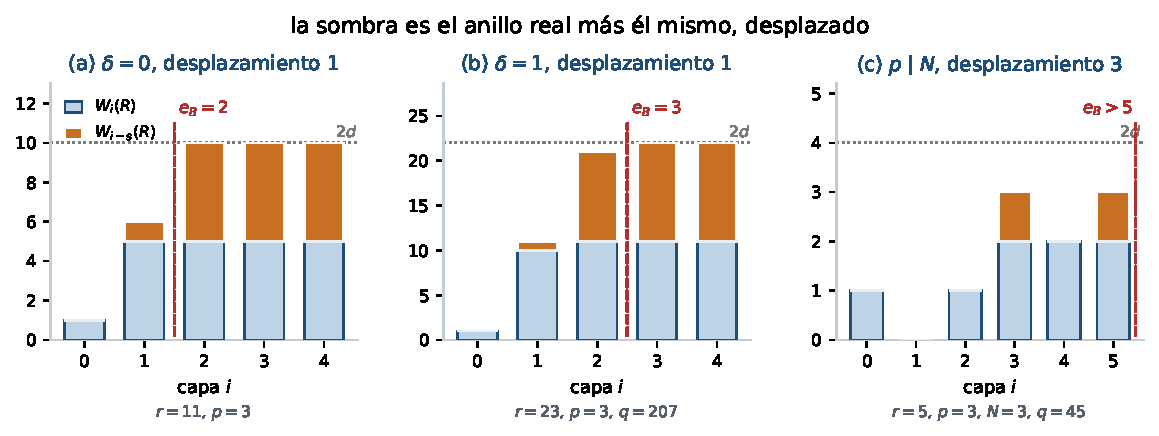
\includegraphics[width=\textwidth]{fig_puente_es.pdf}
\caption{El Teorema~\ref{obs:puente} como una aritm\'etica de barras: la barra clara es $W_i(R)$, la
oscura es la misma barra movida $P$ lugares a la derecha, y la altura total es $W_i(B)$. La l\'inea
de puntos es la dimensi\'on llena $2d$; el exponente del conductor de la sombra es la primera capa
desde la cual las dos barras juntas la alcanzan, que es $P$ m\'as que para $R$ sola --- eso es
$e_B=e_R+P$, visto en vez de cre\'ido. (a) el caso gen\'erico. (b) el primer conductor donde $h^-$
muerde, $r=23$ en $p=3$: el anillo real pierde una dimensi\'on en la capa $1$, la sombra la pierde
dos veces, con una capa de diferencia, y el conductor pasa del cuadrado del radical a su cubo. (c)
cuando $p\mid N$ el desplazamiento es $P=p^{v_p(N)}$ y la barra clara tiene la forma de escalera
del Teorema~\ref{thm:escalera}; aqu\'i la ventana se detiene en $K=6$ antes de que las barras se llenen, de
modo que la marca es una cota y no un valor.}
\label{fig:puente}
\end{figure}

\begin{proposition}[el tipo cruza el puente]\label{prop:tipopuente}
Bajo las hip\'otesis del Teorema~\ref{obs:puente},
$\operatorname{type}(B)=\operatorname{type}(R)$. Si adem\'as $p\nmid N$ y $d/2<u<d$, entonces
$\operatorname{type}(B)=\delta+\kappa-1$ con $\kappa$ como en \cite[Prop.~11]{Cond}; en particular
$B$ es Gorenstein exactamente cuando $\delta=\kappa=1$, aunque su conductor sea una potencia ($P=1$) m\'as
profundo que el de $R$.
\end{proposition}

\begin{proof}
$B$ es libre, luego plano, sobre el anillo local $R$, y $\theta^2$ est\'a en el ideal maximal de
$R$ porque tiene valuaci\'on $2P\ge2$, de modo que la fibra cerrada es $\FF_p[T]/(T^2)$, que es
Gorenstein de tipo $1$. Para un homomorfismo local plano con fibra cerrada Gorenstein el m\'odulo
can\'onico es el cambio de base del m\'odulo can\'onico, as\'i que el tipo queda multiplicado por
el de la fibra \cite[\S3.3]{BH}; los cuerpos residuales coinciden. El segundo enunciado es
\cite[Prop.~11]{Cond} aplicado a $R$, que tiene all\'i $e_R=2$: con $p\nmid N$ se tiene
$W_1(R)=u$, y $d/2<u<d$ es la hip\'otesis de esa proposici\'on.
\end{proof}

Un conductor que es el cuadrado del radical no hace Gorenstein a $R$. Con
$\ell(\cO_+/R)=\sum_{i<e}(d-W_i)$ y $\ell(R/\mathfrak f_R)=\sum_{i<e}W_i$, la condici\'on de
Gorenstein $\ell(\cO_+/R)=\ell(R/\mathfrak f_R)$ se lee $\sum_{i<e}W_i=ed/2$, que es una
condici\'on aparte.

\medido{En $r=41$, $p=11$, $q=451$, $N=1$ el perfil real es $(1,18,20,20)$, as\'i que $e_R=2$ y el
conductor real es el cuadrado del radical, mientras $\ell(\cO_+/R)=21\neq19=\ell(R/\mathfrak f_R)$:
$R$ no es Gorenstein, y por la Proposici\'on~\ref{prop:tipopuente} tampoco lo es $B$, cuyo
conductor es el cubo.}

\medskip
\begin{center}\small
\rowcolors{2}{filaclara}{white}
\begin{tabular}{@{}lllcrr@{}}
\toprule
 & $W(R)$ & $W(B)$ & $e_R\to e_B$ & $v_p([\cO_+:R])$ & $v_p([\cO:B])$ \\
\midrule
$\delta=0$ & $(1,d,d,\dots)$ & $(1,d{+}1,2d,2d,\dots)$ & $1\to2$ & $d-1$ & $3d-2$ \\
$\delta>0$ & $(1,d{-}\delta,d,\dots)$ & $(1,d{+}1{-}\delta,2d{-}\delta,2d,\dots)$ & $2\to3$ &
  $2d-1-u$ & $3d-2+2\delta$ \\
\midrule
$q=207$, $p=3$ & $(1,10,11,\dots)$ & $(1,11,21,22,\dots)$ & $2\to3$ & $11$ & $33$ \\
$q=279$, $p=3$ & $(1,14,15,\dots)$ & $(1,15,29,30,\dots)$ & $2\to3$ & $15^\dagger$ & $45^\dagger$ \\
\bottomrule
\end{tabular}
\end{center}

\noindent{\small El puente en dos reg\'imenes y en las \'unicas dos casillas del rango barrido con
$\delta>0$, las dos con $r$ primo y $p=3\mid h^-$ y $\delta=1$. Las capas est\'an medidas; los dos
\'indices en $q=207$ son ret\'iculos enteros cerrados, y los dos marcados con $\dagger$ son la ley
aplicada a las capas medidas, no ret\'iculos. En $q=207$ el plano de la \S\ref{sec:loc} dar\'ia
$32$.}
\medskip

\medido{Comprobaciones independientes:
las identidades mostradas valen en $306$ de $306$ casillas le\'idas a profundidad $K=\min(E,4)$, la
ley del \'indice en $13$ de $13$ casillas cerrando ret\'iculos enteros en vez de capas, y los siete
pasos de la demostraci\'on --- el representante, la unidad, $\mu\in B$, $B=A[\mu]$, $R=A$,
$B^-=\theta R$ y $v_p(\theta)=P$ --- cada uno por separado en $66$ de $66$ casillas con
ret\'iculos enteros localizados en $p$, con $P=1$, $3$ y $9$, con $\varphi(p^v)=2$, con $r$
compuesto y con $N\le9$. Cada uno de los siete est\'a cubierto por la demostraci\'on.}

Tres observaciones sobre lo que la demostraci\'on \emph{no} usa. No necesita $E\ge3$: nada se
desarrolla a segundo orden en $\pi$. Ni ella ni la Proposici\'on~\ref{prop:tau} necesitan
$u>d/2$; esa hip\'otesis entra s\'olo a trav\'es de lo que \cite{Cond} puede decir
del perfil del anillo real, que es lo que fija $e_R\le2$ y con ello la f\'ormula mostrada. Y no
nombra un anillo simpl\'ectico: $R$ es el anillo del segmento centrado, y la identificaci\'on de
ese anillo con $A_{\Sp(2m)}(q)$ para un $m$ adecuado es la Proposici\'on~\ref{prop:ops} y el
Corolario~\ref{cor:par} aplicados a $S-Nr/2$, cuya longitud es $Nr\pm1$ --- as\'i que $m$ depende
de $N$, y la conjetura ingenua $m=r-1$ falla incluso localmente: en $q=45$, $p=3$, $N=3$ el anillo $R$
tiene $v_3([\cO_+:R])=4$ y $W_1(R)=0$, mientras que $A_{\Sp(8)}(45)$ tiene $v_3=1$ y $W_1=2$. Sobre $9$ casillas y
$54$ comparaciones, $A_{\Sp(2m)}(q)$ con $m=r-1$, $m=r$ y $m=(q-r-2)/2$ dan la misma imagen
truncada mientras que $m=r-2$ y $m=r+1$ no, y $m=r-3$ s\'olo en las dos casillas de $q=45$, y los
ret\'iculos enteros de los tres ya son distintos en $q=45$, de \'indices $75$, $3$ y $3$.

Lo que mide el desplazamiento es el grado del generador antiinvariante, y ese grado tiene una
lectura propia. Escr\'ibase $n'$ para aquel de $n$, $n-1$ que sea divisible por $r$; entonces
$P=v_p(\zeta_q^{\,n'}-1)$ es lo lejos que est\'a el segmento de cerrar un per\'iodo completo.
Cuando lo cierra, $\zeta_q^{\,n'}=1$ y la extensi\'on degenera --- que es la otra cosa que esta
secci\'on ya sab\'ia, $B_n(q)=\ZZ$ en $n\equiv0,1\pmod q$. Un solo n\'umero gobierna los dos
extremos.

La forma del Teorema~\ref{obs:puente} no es nueva: si un orden de un cuerpo CM es libre de rango dos
sobre el subanillo fijo por la conjugaci\'on compleja es una hip\'otesis que Howe aisl\'o y us\'o
\cite[pp.~13, 20]{Howe}, y, en el marco CM cu\'artico de \cite{IT}, cuando el anillo real es el
\emph{maximal} el conductor de una extensi\'on as\'i est\'a calculado y el orden es Gorenstein por
ser monog\'enico \cite[Lemmas 7, 8]{IT} --- un precedente de forma, no una demostraci\'on para
\'ordenes ciclot\'omicos de grado arbitrario. La consecuencia graduada tiene tambi\'en una forma
est\'andar: para \'algebras graduadas artinianas, $\gr(B)$ sobre $\gr(R)$ con fibra
$\FF_p[\bar\theta]/(\bar\theta^2)$ es una \emph{extensi\'on libre} en el sentido de Harima y
Watanabe, cuya funci\'on de Hilbert se multiplica \cite[Def.~1.5, Lem.~1.6]{IM}. Nuestros anillos
graduados no son artinianos, as\'i que citamos esto como contexto: aqu\'i el producto de series de
Hilbert se demuestra por la suma directa filtrada de la demostraci\'on de arriba, no por
\cite{IM}. Lo nuevo es qu\'e \'ordenes son \'estos, y
que el real no es maximal: all\'i las capas de $R$ no est\'an todas llenas y la convoluci\'on tiene
contenido.

\frontera{\textbf{D\'onde s\'i se rompe.} No en $p\mid N$: nada en la demostraci\'on mira a $N$
m\'odulo $p$, y lo \'unico que cambia all\'i es el valor de $P$. Se rompe en $p=2$: el m\'odulo $q$ es par
y $2^{-1}$ no existe m\'odulo $q$. El elemento de centrado puede existir a\'un cuando $Nr$ es par
--- $q=20$, $r=5$, $N=2$ tiene $\mu=\zeta_{20}^{\,5}$ ---, pero la demostraci\'on recupera $\mu$ de
$\mu^2$ a trav\'es de su orden impar y parte $B$ con los proyectores $(1\pm\iota)/2$, y los dos
pasos dividen por $2$. \'Ese es un problema distinto, no un caso m\'as dif\'icil de \'este --- el
\'indice $2^7$ en $(n,q)=(7,14)$, registrado y sin explicar tras el Teorema~\ref{thm:sombra}, es su
instancia m\'as peque\~na. Para $u\le d/2$ el anillo sigue siendo $A$, por la
Proposici\'on~\ref{prop:tau}, pero \cite{Cond} no da all\'i el perfil de $A$, de modo que el $W(B)$
mostrado no se sigue. \'Esa es una laguna en el insumo real, no en el
puente.}

\section{Dos fronteras}

\frontera{\textbf{El criterio de $h^-$ en la sombra, fuera del puente.} En $q'=31$ con $n=q'$ el
defecto real es $3$ mientras que la sombra cae en $1$: los dos no se est\'an comparando contra el
mismo anillo. El Teorema~\ref{obs:puente} dice contra qu\'e anillo real hay que comparar la sombra
--- no el del mismo $n$, sino el del segmento recentrado en $Nr/2$, cuyo defecto all\'i es tambi\'en
$1$ --- y eso es lo que disuelve la asimetr\'ia dentro de la familia principal. Lo abierto est\'a
fuera de ella. Cuando $p\mid N$ --- la segunda fuente de defecto, ya presente en el tipo $C$ --- la
demostraci\'on \emph{no} se detiene: $e_1(S)$ sigue siendo unidad, viniendo el residuo $\pm1$ de la
suma sobre todas las clases y no de $N$, y lo \'unico que cambia es que el desplazamiento pasa a
ser $p^{v_p(N)}$. Lo abierto all\'i es m\'as estrecho, y no es un paso: el anillo fijo $B^\iota$
es $A$ por la Proposici\'on~\ref{prop:tau}, el anillo del segmento centrado $S-Nr/2$, que la
\S\ref{sec:seg} identifica con un anillo simpl\'ectico; lo que no est\'a zanjado cuando $p\mid N$
es su perfil m\'as all\'a de la profundidad $P$; por debajo de ella ese anillo sigue la escalera
(Teorema~\ref{thm:escalera}). Para la primera capa de la sombra la pregunta no se plantea: la
Proposici\'on~\ref{prop:capa1} la responde directamente, y la respuesta es $W_1=0$. Y $p=2$ es un
problema distinto: $q$ es par, $2^{-1}$ no existe m\'odulo $q$, e incluso donde existe un
elemento de centrado la recuperaci\'on de $\mu$ a partir de $\mu^2$ y los proyectores de la
demostraci\'on dividen por $2$. El enunciado hay que hacerlo familia por familia, como en \cite{Cond}, y no de una
pieza.}

\frontera{\textbf{La lectura estratificada, y la conjetura que mata.} Las columnas las permutan los
estratos $X_D=\{c:\gcd(c,q')=D\}\cong(\ZZ/(q'/D))^\times$, que es la estructura de los
\emph{grafos de mcd}, cuyos autovalores son sumas de Ramanujan y que por el teorema de So son los
\'unicos grafos circulantes enteros \cite{So,KS}. Escribiendo $S_D$ para la restricci\'on de $S$ a
$X_D$, el anulador se parte, $\operatorname{Ann}(S)=\bigcap_D\operatorname{Ann}(S_D)$, de modo que
\[
\marco{W_1=\operatorname{codim}_{\FF_p[G]}\ \bigcap_{D\mid q'}\operatorname{Ann}(S_D),\qquad
G=(\ZZ/q')^\times,}
\]
que es la lectura estratificada en su forma correcta: cuando $p\nmid\varphi(q')$ el \'algebra de
grupo es semisimple y un bloque cuenta una vez, en cuanto sobrevive en \emph{al menos un} estrato.
Sumar los estratos en su lugar lo cuenta una vez por estrato, que es por lo que eso se pasa.
Lo que no funciona es el refinamiento que uno quiere a continuaci\'on. Un car\'acter de conductor
$f$ aparece en todo estrato con $f\mid q'/D$, as\'i que uno espera que o sobrevive en todos o en
ninguno, lo que har\'ia de $\operatorname{codim}\operatorname{Ann}(S_D)$ una suma de divisores en
$q'/D$ y dar\'ia un recuento por conductor. Es falso: la supervivencia depende del estrato, y en
$76$ de $416$ casillas estables ni siquiera el estrato de las unidades $D=1$, el mayor, ve la
primera capa entera. Un testigo con \'algebra de grupo semisimple est\'a en la sombra, el segmento
$\{0,\dots,13\}$ de $\GL(14)$ en $q'=14$, $p=5$ ($q=70$, y $5\nmid\varphi(14)$), donde la dimensi\'on de capa es $\varphi(14)=6$, $W_1=4$ y
$\operatorname{codim}\operatorname{Ann}(S_1)=3$: un bloque muere en las unidades y vive en un
estrato menor. As\'i que un recuento por conductor que suponga que un bloque sobrevive
uniformemente a trav\'es de los estratos es falso; una clasificaci\'on por conductor que lleve los
datos de los estratos no queda descartada, y lo que falta es una descripci\'on de en qu\'e estratos
sobrevive un bloque.}

\begin{remark}[un resultado negativo]
$\gr_1(A)$ \emph{no} es la \'orbita de Galois de un solo elemento de $\bar R$: es la envolvente de
todos los coeficientes de un polinomio. Tres intentos de describirlo as\'i --- el m\'odulo generado
por $\sum_cS(c)\omega^c$, la suma de los rangos estrato a estrato, y el m\'odulo generado por
$\sum_cS(c)U_c\omega^c$ --- dan $181$, $169$ y $101$ de las $193$ casillas estables, frente a $193$
de la matriz del Teorema~\ref{thm:loc}.
\end{remark}

\section{Qu\'e calcula esto, y una herramienta que lo calcula}\label{sec:util}

Dos de los enunciados anteriores sustituyen un c\'alculo por una f\'ormula, y eso conviene decirlo
en la moneda de quien tiene que hacer el c\'alculo. El objeto es un orden de un cuerpo
ciclot\'omico y la pregunta es su conductor; \'esa es la tarea de cada d\'ia en la algor\'itmica de
la multiplicaci\'on compleja, donde el conductor de un orden CM es lo que uno calcula para
identificar un anillo de endomorfismos o para situar una curva en un grafo de isogenias
\cite{IT,BSt13}. En ese contexto los dos se leen as\'i.

\emph{Un filtro que no cuesta nada.} El Teorema~\ref{thm:sop} dice que $p$ s\'olo puede dividir a
$[\cO:A]$ cuando $r$ divide a uno de $n-1,n,n+1$, y el Corolario~\ref{cor:sopsombra} lo estrecha a
$n,n-1$ en la sombra. Eso es una prueba de divisibilidad: sin ret\'iculo, sin matriz, sin capas.
Certifica la maximalidad en todo primo fuera de las familias en lo que se tarda en reducir $n$
m\'odulo $r$,
y puede correrse sobre tantos pares como uno quiera antes de empezar el
trabajo de verdad.

\emph{La mitad del grado.} El Teorema~\ref{obs:puente} da
$v_p([\cO:B_n])=2\,v_p([\cO_+:R])+P\,d$. El lado izquierdo es un invariante de un orden de grado
$\varphi(q)$; el derecho se calcula en el subcuerpo real, de grado $\varphi(q)/2$, m\'as una
multiplicaci\'on. \'Esta es la forma de enunciado que la literatura de CM tiene para el caso en que
el orden real es \emph{maximal} \cite[Lemmas 7, 8]{IT}; lo nuevo es que no lo necesita.

La herramienta implementa adem\'as, como \texttt{ceros} y \texttt{fila}, los dos recuentos de la
nota compa\~nera \cite{II}: las componentes que se anulan en la diagonal, y las filas que ocupa
un car\'acter cuadr\'atico --- exactamente las de $\bigl(\frac2n\bigr)=1$, que \cite{II} demuestra
probando que en toda longitud admisible existe un patr\'on de signos completamente multiplicativo con
suma pesada nula.

\paragraph{La herramienta.} \texttt{segmento.py} viaja con esta nota: un fichero, s\'olo biblioteca
est\'andar de Python~3, sin instalaci\'on y sin sistema de \'algebra computacional. Expone
\texttt{familias}, \texttt{perfil}, \texttt{indice}, \texttt{puente}, \texttt{ceros} y
\texttt{fila} --- una rutina por enunciado de esta nota y de \cite{II}, con su nombre --- como
biblioteca y como l\'inea de \'ordenes, junto con \texttt{segmento\_SU}, que devuelve el segmento de
$g_q$ con su m\'odulo ($M=2q$ para $n$ par, como en la \S\ref{sec:seg}). Ejecutar \texttt{python segmento.py autotest} reproduce,
desde cero, los ejemplos resueltos de esta nota --- los perfiles $(1,11,21,22)$ en $q=207$ y
$(1,15,29,30)$ en $q=279$, el \'indice $v_3([\cO:B_{23}(207)])=33$ --- y los de \cite{II}. El camino lento, \texttt{indice}, se conserva a prop\'osito: es el control contra
el que se comprueban las f\'ormulas, y la comprobaci\'on forma parte de la prueba. Est\'a adem\'as
depositada por su cuenta, bajo CC0 y con DOI propio \cite{Tool}, para que pueda encontrarla, usarla
y citarla quien nunca lea esta nota --- que es el p\'ublico que tiene una aplicaci\'on.

\medido{El atajo contra el camino lento en $9$ casillas con $\varphi(q)\le132$: el mismo entero en
cada casilla, y alrededor de la mitad del reloj en la mayor de ellas. El factor es el cociente de
los dos grados y no una afirmaci\'on asint\'otica --- las dos rutas corren el mismo c\'odigo de
capas, y la \'unica diferencia es que una cierra en grado $\varphi(q)$ y la otra en $\varphi(q)/2$;
los tiempos mismos son una propiedad de la m\'aquina y la corrida archivada los registra. El guion
que los cronometra, \texttt{medir\_atajo.py}, viaja tambi\'en con la nota.}

\noindent Lo que la herramienta \emph{no} hace es ocultar el suelo de honestidad de la nota: all\'i
donde un enunciado est\'a medido y no demostrado --- el recuento de componentes que se anulan en
un $f$ compuesto, donde ese recuento exige $f$ primo --- la rutina correspondiente lo dice y
declina; y all\'i donde el perfil de capas se corta a profundidad $E$ antes de llenarse,
\texttt{indice} y \texttt{puente} devuelven una cota inferior y lo dicen; y en $q'\le2$, fuera del
Teorema~\ref{thm:loc}, \texttt{indice} declina. Las guardas son exactamente esas tres y ninguna
m\'as. El atajo no est\'a guardado en $u\le d/2$, porque la
Proposici\'on~\ref{prop:tau} da $R=A$ sin condiciones; y no est\'a guardado en $p\mid N$, y
no debe estarlo, porque all\'i el n\'umero s\'i est\'a justificado y lo que queda abierto es el
perfil m\'as profundo del lado real, no un paso.

\section*{MSC 2020}
Primary 11R18; Secondary 11R29, 11R04, 13H10, 13B22, 05C50, 20G05, 11Y40.

\section*{Declaraci\'on de conflicto de intereses}
El autor declara no tener conflicto de intereses ni financiaci\'on.

\section*{Disponibilidad de los datos}
No se han usado datos externos. Los datos computacionales --- cada n\'umero etiquetado como
\emph{medido}, y cada figura --- los generan guiones que viajan con esta nota junto con su salida
archivada. Entre ellos est\'a \texttt{segmento.py} de la \S\ref{sec:util}, un \'unico fichero sin
dependencias que implementa los enunciados de esta nota y verifica sus propios n\'umeros con
\texttt{python segmento.py autotest}; se publica en el dominio p\'ublico bajo CC0 para que pueda
usarse, trocearse o reescribirse sin pedir permiso, y est\'a depositado como registro de software
citable por s\'i mismo \cite{Tool}.

\section*{Declaraci\'on sobre IA generativa}
Esta nota se ha escrito con Claude (Anthropic) como asistente, bajo la direcci\'on del autor. Todo
enunciado marcado como \emph{medido} lo produce un guion archivado con la nota; el autor es
responsable del contenido.

\begin{thebibliography}{99}
\bibitem{BS} A.~B\"achle, B.~Sambale, \emph{Orders generated by character values},
Monatsh.~Math.~\textbf{191} (2020), 665--678.
\bibitem{BSt13} G.~Bisson, M.~Streng, \emph{On polarised class groups of orders in quartic
CM-fields}, Math.~Proc.~Cambridge Philos.~Soc.~\textbf{163} (2017), 233--254,
\href{https://arxiv.org/abs/1302.3756}{\texttt{arXiv:1302.3756}}.

\bibitem{CMP} P.~Cellini, P.~M\"oseneder Frajria, P.~Papi, \emph{The $\widehat W$-orbit of $\rho$,
Kostant's formula for powers of the Euler product and affine Weyl groups as permutations of
$\mathbb{Z}$}, J.~Pure Appl.~Algebra \textbf{208} (2007), 1103--1119;
\texttt{arXiv:math/0507610}.
\bibitem{Ded77} R.~Dedekind, \emph{\"Uber die Anzahl der Ideal-Klassen in den verschiedenen Ordnungen
eines endlichen K\"orpers}, Festschrift der Technischen Hochschule Braunschweig, Vieweg (1877),
1--55.
\bibitem{FSS} J.~Fuchs, A.~N.~Schellekens, C.~Schweigert, \emph{From Dynkin diagram symmetries to
fixed point structures}, Comm.~Math.~Phys.~\textbf{180} (1996), 39--97.
\bibitem{Hopper} J.~Hopper, \emph{The twining character formula for reductive groups},
\texttt{arXiv:2204.03600}.
\bibitem{Jan} J.~C.~Jantzen, \emph{Darstellungen halbeinfacher Gruppen und kontravariante Formen},
J.~reine angew.~Math.~\textbf{290} (1977); the twining character formula goes back to his 1973 work.
\bibitem{Howe} E.~W.~Howe, \emph{Kernels of polarizations of abelian varieties over finite fields},
J.~Algebraic Geom.~\textbf{5} (1996), 583--608; page numbers as in the reproduction of the 1995
preprint, \href{https://arxiv.org/abs/2001.05111}{\texttt{arXiv:2001.05111}}.

\bibitem{IM} A.~Iarrobino, P.~Macias Marques, C.~McDaniel, \emph{Artinian Gorenstein algebras that
are free extensions
over $k[t]/(t^n)$, and Macaulay duality}, J.~Pure Appl.~Algebra \textbf{224} (2020), 106305,
\href{https://arxiv.org/abs/1807.02881}{\texttt{arXiv:1807.02881}}; free extensions are due to
T.~Harima and J.~Watanabe.

\bibitem{IT} S.~Ionica, E.~Thom\'e, \emph{Isogeny graphs with maximal real multiplication},
J.~Number Theory \textbf{207} (2020), 385--422,
\href{https://arxiv.org/abs/1407.6672}{\texttt{arXiv:1407.6672}}; Lemma~7 is due to E.~Goren and
K.~Lauter, and Lemma~8 rests on J.~Buchmann and H.~W.~Lenstra, \emph{Approximating rings of
integers in number fields}, J.~Th\'eor.~Nombres Bordeaux \textbf{6} (1994), 221--260, (2.7)--(2.8).

\bibitem{KS} W.~Klotz, T.~Sander, \emph{Some properties of unitary Cayley graphs},
Electron.~J.~Combin.~\textbf{14} (2007).
\bibitem{Kostant76} B.~Kostant, \emph{On Macdonald's $\eta$-function formula, the Laplacian and
generalized exponents}, Adv.~Math.~\textbf{20} (1976), 179--212.
\bibitem{Kostant04} B.~Kostant, \emph{Powers of the Euler product and commutative subalgebras of a
complex simple Lie algebra}, Invent.~Math.~\textbf{158} (2004), 181--226.
\bibitem{Cond} C.~Mar\'in, \emph{Where the character values of $\Sp(2m)$ at a torsion element fail
to generate the ring of integers}, \href{https://doi.org/10.5281/zenodo.22813216}{\texttt{doi:10.5281/zenodo.22813216}}, 2026.
\bibitem{Tool} C.~Mar\'in, \emph{Computing the conductor and index of orders generated by
character values: an exact, dependency-free Python tool for $\SU(n)$, $\Sp(2m)$ and $\GL(n)$
(\texttt{segmento.py})}, software, v1.0.0, CC0,
\href{https://doi.org/10.5281/zenodo.22834098}{\texttt{doi:10.5281/zenodo.22834098}}, 2026.
\bibitem{Des82} J.~D\'esarm\'enien, \emph{Un analogue des congruences de Kummer pour les
$q$-nombres d'Euler}, European J.~Combin.~\textbf{3} (1982), 19--28.

\bibitem{Oli65} G.~Olive, \emph{Generalized powers}, Amer.~Math.~Monthly \textbf{72} (1965),
619--627.

\bibitem{Sag92} B.~E.~Sagan, \emph{Congruence properties of $q$-analogs}, Adv.~Math.~\textbf{95}
(1992), 127--143; the $q$-Lucas theorem is Theorem~2.2, with its history on p.~131.

\bibitem{NS07} S.~G.~Naculich, H.~J.~Schnitzer, \emph{Level-rank duality of the $U(N)$ WZW model,
Chern--Simons theory, and 2d qYM theory}, JHEP \textbf{0706} (2007) 023,
\href{https://arxiv.org/abs/hep-th/0703089}{\texttt{arXiv:hep-th/0703089}}.

\bibitem{NT92} T.~Nakanishi, A.~Tsuchiya, \emph{Level-rank duality of WZW models in conformal field
theory}, Comm.~Math.~Phys.~\textbf{144} (1992), 351--372.

\bibitem{ABI90} D.~Altschuler, M.~Bauer, C.~Itzykson, \emph{The branching rules of conformal
embeddings}, Comm.~Math.~Phys.~\textbf{132} (1990), 349--364.

\bibitem{SA91} H.~Saleur, D.~Altschuler, \emph{Level-rank duality in quantum groups},
Nucl.~Phys.~B \textbf{354} (1991), 579--613.

\bibitem{MNRS91} E.~J.~Mlawer, S.~G.~Naculich, H.~A.~Riggs, H.~J.~Schnitzer, \emph{Group-level
duality of WZW fusion coefficients and Chern--Simons link observables}, Nucl.~Phys.~B \textbf{352}
(1991), 863--896.

\bibitem{Fre82} I.~B.~Frenkel, \emph{Representations of affine Lie algebras, Hecke modular forms and
Korteweg--de Vries equations}, in Lie Algebras and Related Topics, Lecture Notes in
Math.~\textbf{933}, Springer, 1982, p.~71.

\bibitem{BH} W.~Bruns, J.~Herzog, \emph{Cohen--Macaulay Rings}, rev.~ed., Cambridge Stud.~Adv.~Math.
\textbf{39}, Cambridge Univ.~Press, 1998.

\bibitem{PS86} A.~Pressley, G.~Segal, \emph{Loop Groups}, Oxford Univ.~Press, 1986; the
$k\leftrightarrow N-k$ symmetry is Proposition~(10.6.4), p.~212, as cited in \cite{Wit93}.

\bibitem{Wit93} E.~Witten, \emph{The Verlinde algebra and the cohomology of the Grassmannian},
\href{https://arxiv.org/abs/hep-th/9312104}{\texttt{arXiv:hep-th/9312104}}; in Geometry, Topology
and Physics, Conf.~Proc.~Lecture Notes Geom.~Topology IV, Int.~Press, 1995, 357--422.

\bibitem{NPP} S.~Nadimpalli, S.~Pattanayak, D.~Prasad, \emph{Character theory at a torsion element},
\texttt{arXiv:2504.14684}.
\bibitem{Pia87} A.~Pianzola, \emph{On the arithmetic of the representation ring and elements of
finite order in Lie groups}, J.~Algebra \textbf{108} (1987), 1--33.
\bibitem{Sin78} W.~Sinnott, \emph{On the Stickelberger ideal and the circular units of a cyclotomic
field}, Ann.~of Math.~\textbf{108} (1978), 107--134.
\bibitem{So} W.~So, \emph{Integral circulant graphs}, Discrete Math.~\textbf{306} (2006), 153--158.
\bibitem{II} C.~Mar\'in, \emph{Zeros of weighted partial sums of completely multiplicative
functions: Dirichlet characters, the Euler factor at $2$ and Conrey's sine series},
\href{https://doi.org/10.5281/zenodo.22847374}{\texttt{doi:10.5281/zenodo.22847374}}, 2026.

\end{thebibliography}

\end{document}
